\typeout{(body.tex)}
\newcommand{\nred}[1]{{\color{red!60!black}\bfseries #1}}
\newcommand{\nred}[1]{\textbf{#1}}


\begin{frame}
    \titlepage
\end{frame}

% Introduction:
    % do we need more than lists?
        % better than linear search
        % complex relationships
            % examples: language tree, phylogenic
    % relationships between nodes
        % list as up to 2
        % binary tree as up to 3
\section{why trees?}
\begin{frame}{are lists enough?}
\begin{itemize}
    \item for correctness --- sure
    \vspace{.5cm}
    \item want to efficiently access items
        \begin{itemize}
        \item \myemph{better than linear time} to find something
        \end{itemize}
    \item want to \myemph{represent relationships} more naturally
\end{itemize}
\end{frame}

\begin{frame}{inter-item relationships in lists}
\begin{tikzpicture}
\tikzset{>=Latex}
\node[draw] (n1) { 1 };
\node[draw,right=1cm of n1] (n2) { 2 };
\node[draw,right=1cm of n2] (n3) { 3 };
\node[draw,right=1cm of n3] (n4) { 4 };
\node[draw,right=1cm of n4] (n5) { 5 };
\foreach \x/\y in {1/2,2/3,3/4,4/5} {
    \draw[ultra thick,<->] (n\x) -- (n\y);
}
\end{tikzpicture}
\begin{itemize}
\item List: \textit{nodes} related to \myemph{predecessor}/\myemph{successor}
\end{itemize}
\end{frame}

\begin{frame}{trees}
\begin{itemize}
    \item trees: allow representing more relationships
        \begin{itemize}
        \item (but not arbitrary relationships --- see graphs later in semester)
        \end{itemize}
    \item restriction: single path from \textit{root} to every node
        \begin{itemize}
        \item implies single path from every node to every other node (possibly through root)
        \end{itemize}
\end{itemize}
\end{frame}

\begin{frame}{natural trees: phylogenetic tree}
\vspace{-.25cm}
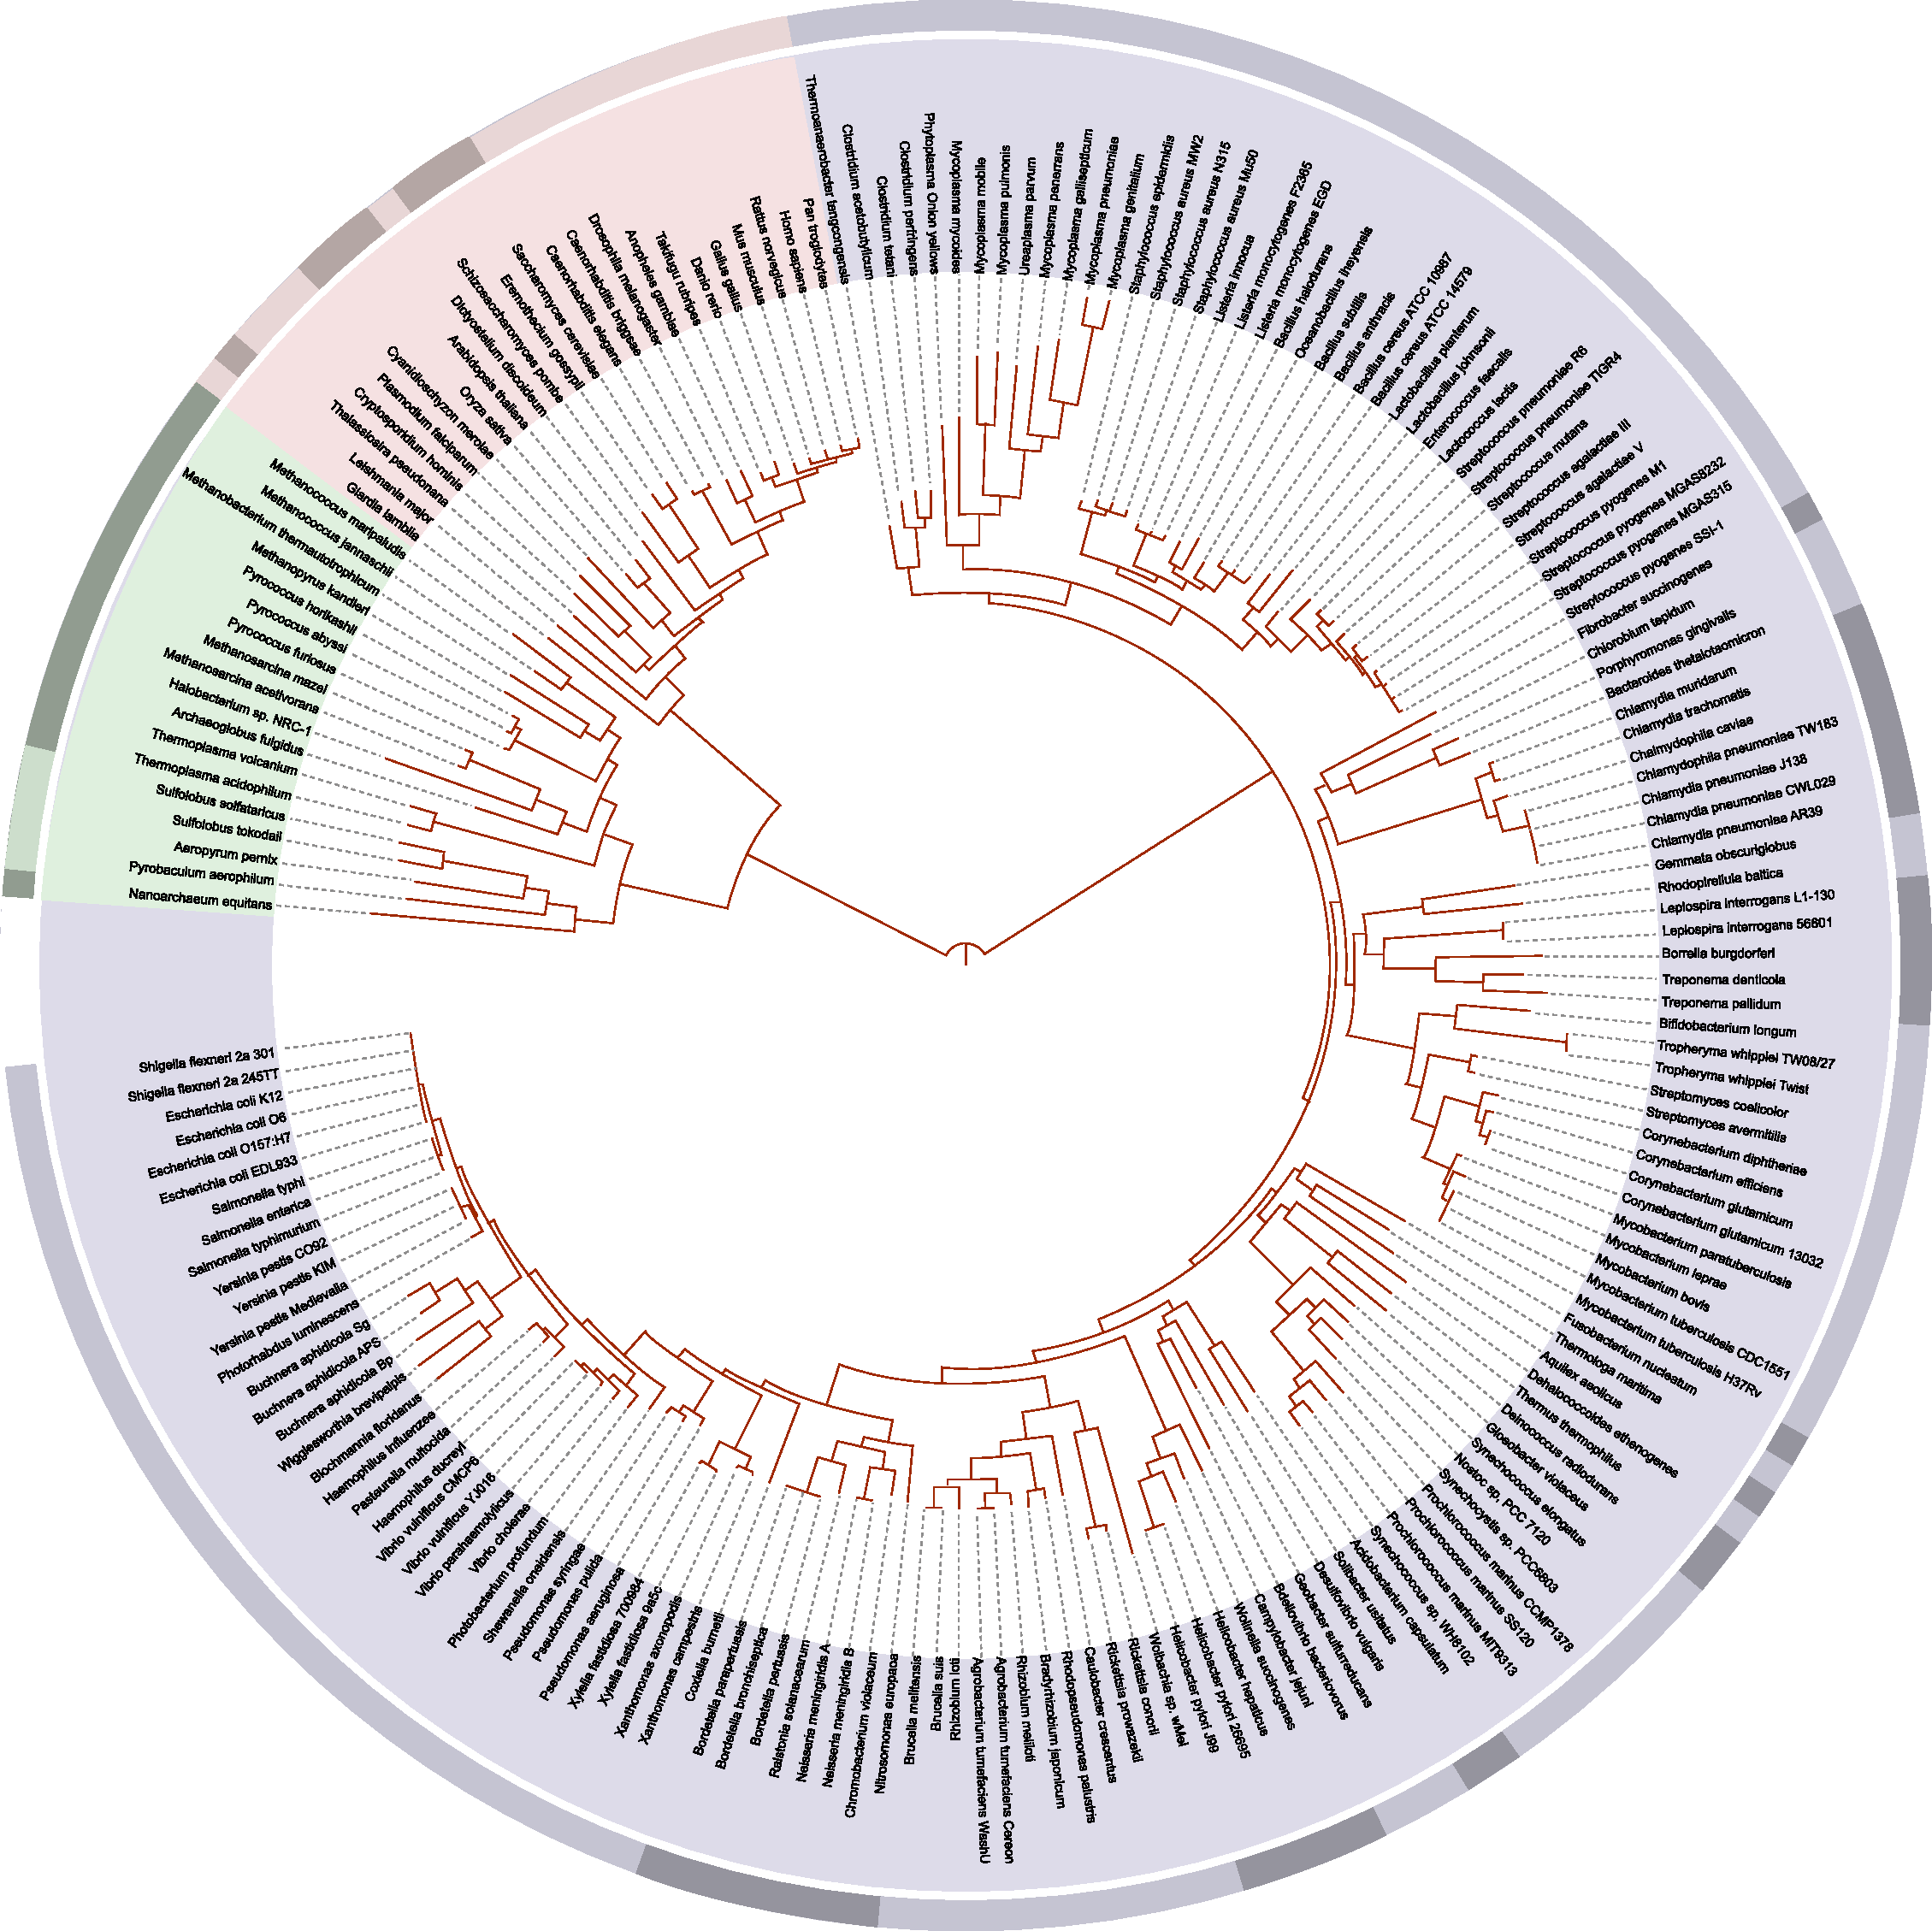
\includegraphics[height=0.9\textheight]{Tree_of_Life}
\imagecredit{image: Ivicia Letunic and Mariana Ruiz Villarreal, via the tool iTOL (Interative Tree of Life), via Wikipedia}
\end{frame}

\begin{frame}{natural trees: phylogenetic tree (zoom)}
\vspace{-.25cm}
    \adjincludegraphics[height=0.9\textheight,trim={{0\width} {0\height} {.25\height} {.6\width}},clip]{Tree_of_Life}
\imagecredit{image: Ivicia Letunic and Mariana Ruiz Villarreal, via the tool iTOL (Interative Tree of Life), via Wikipedia}
\end{frame}

\begin{frame}{natural trees: Indo-European languages}
\vspace{-.25cm}
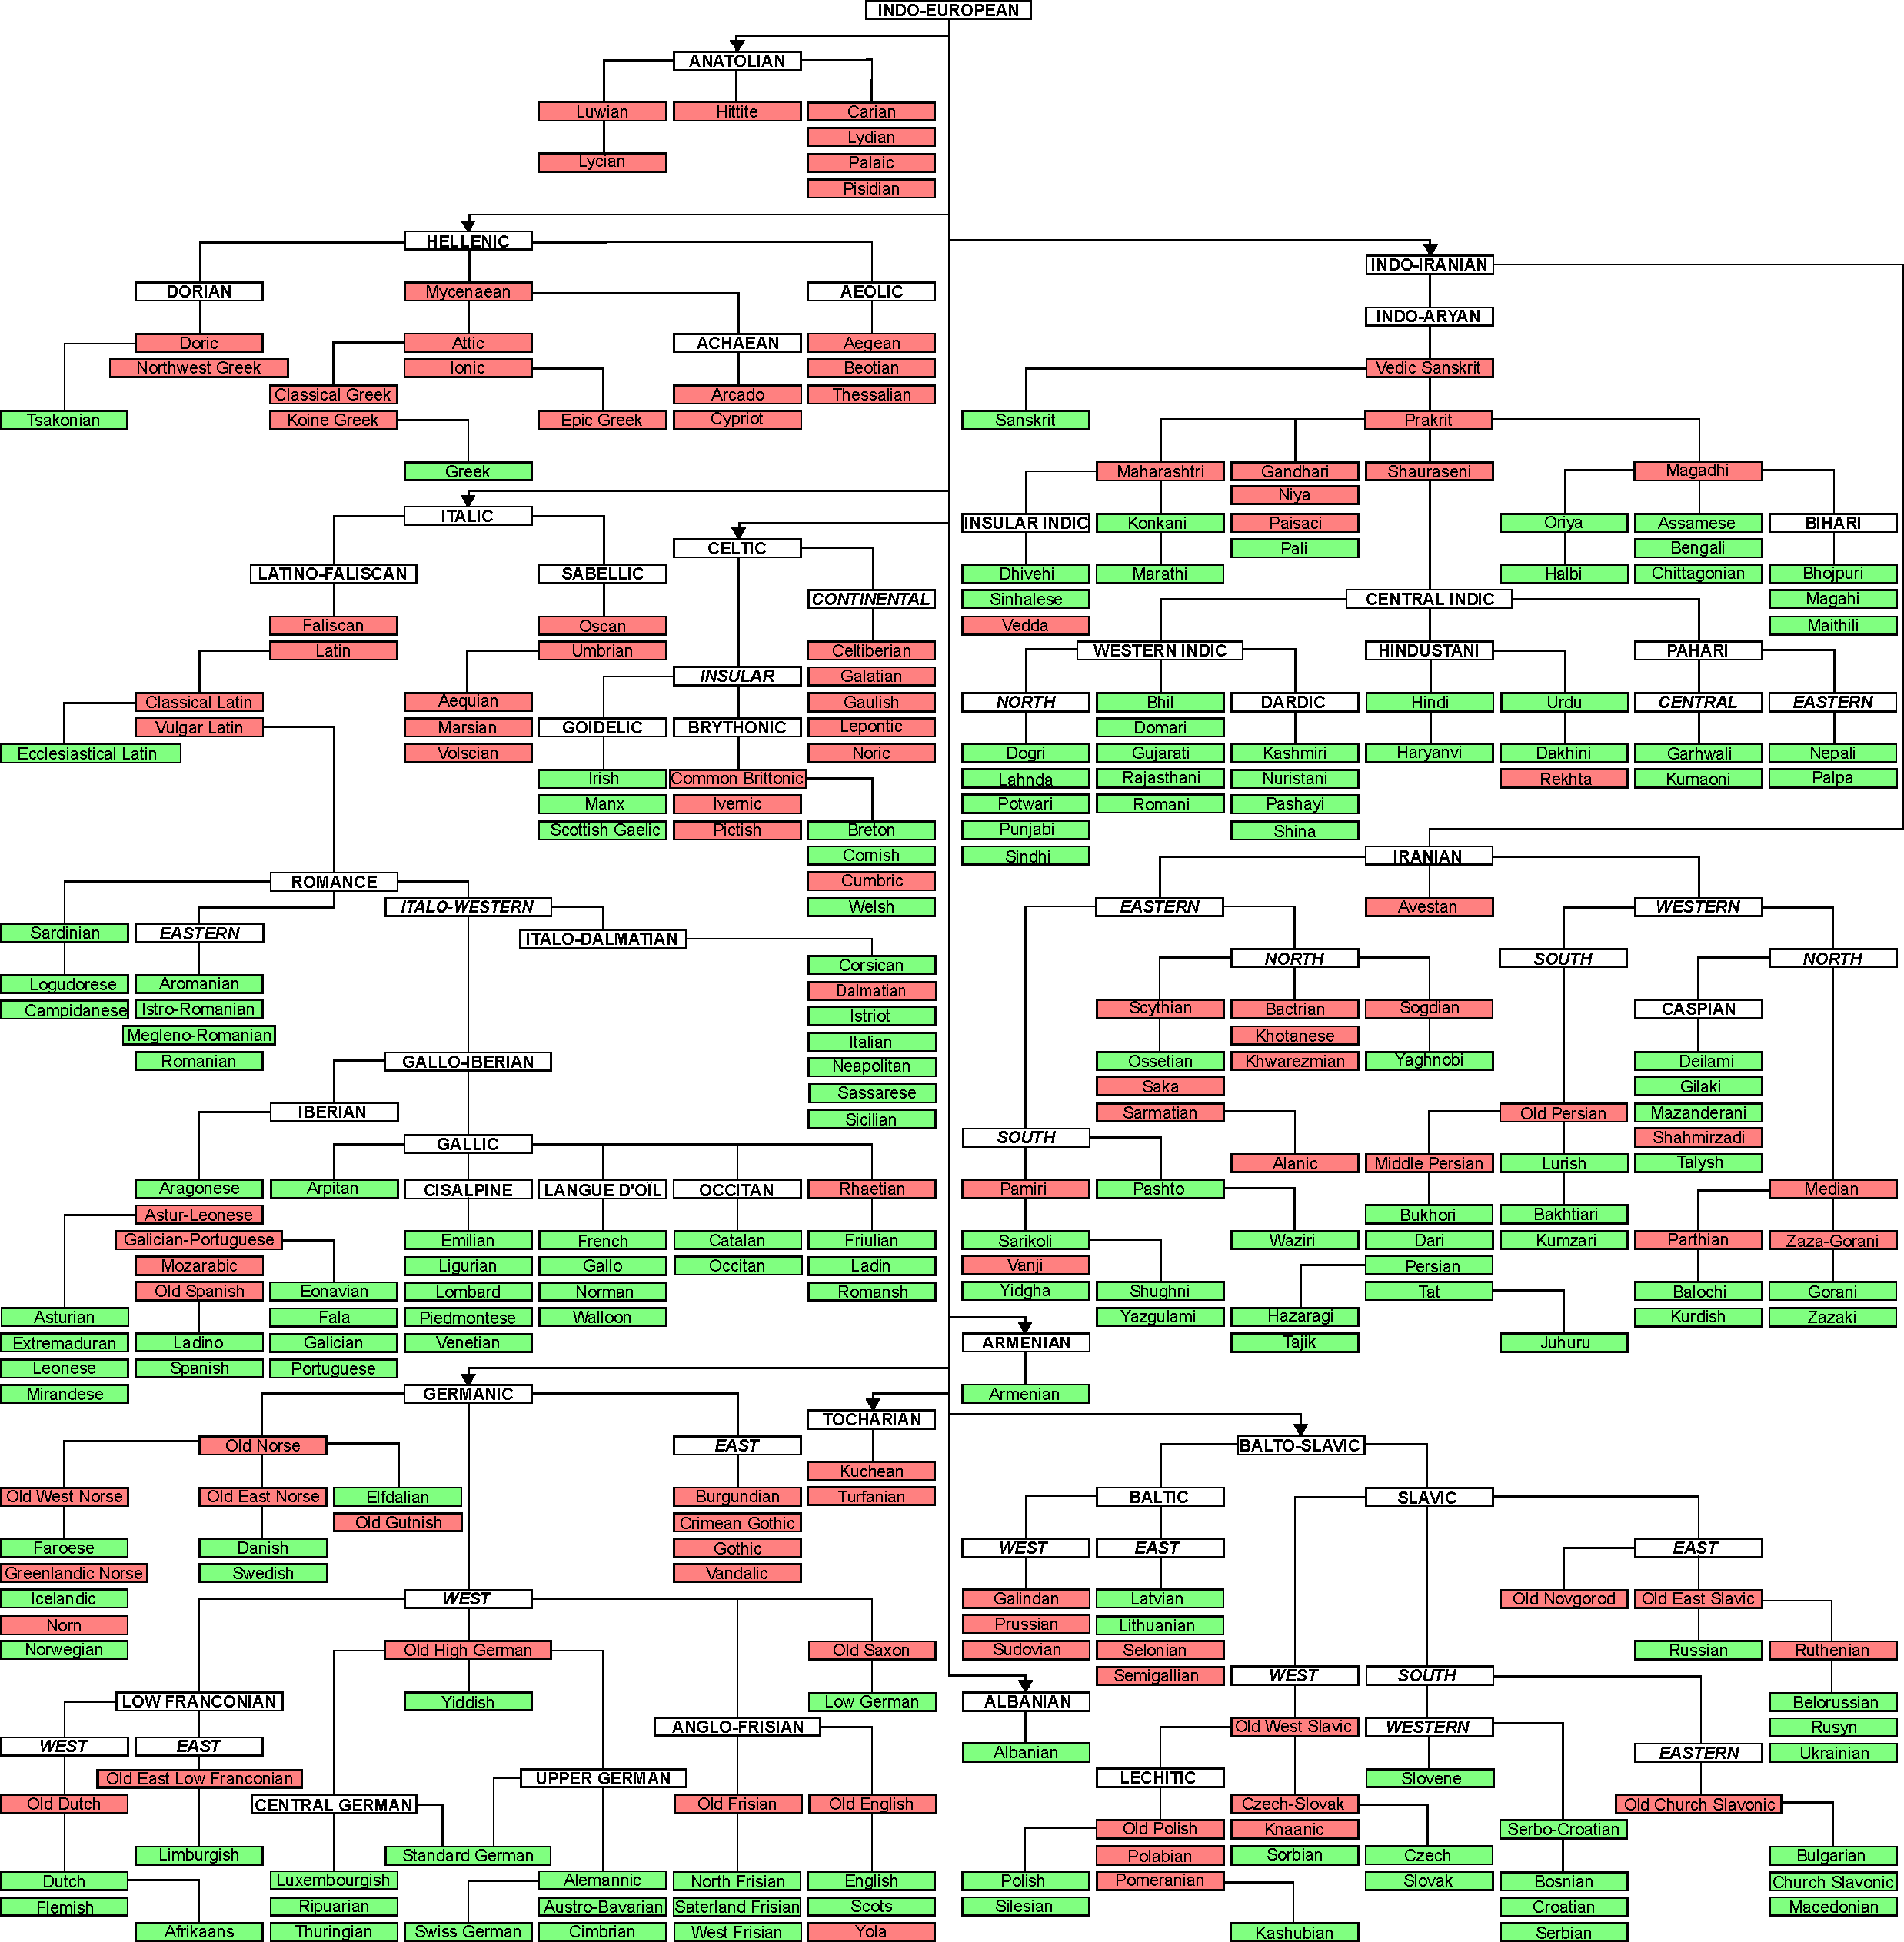
\includegraphics[height=0.9\textheight]{IndoEuropeanTree}
\imagecredit{image: via Wikipedia/Mandrak}
\end{frame}

\begin{frame}{list to tree}
\begin{tikzpicture}
\tikzset{>=Latex}
\begin{scope}[start chain=going right,every join/.style={->,very thick}]
\node[draw,thick,on chain] {predecessor};
\node[draw,thick,on chain,join] (elem) {element};
\node[draw,thick,on chain,join] {successor};
\end{scope}
\node[above=.5cm of elem] {\textit{list} --- up to 2 related nodes};

\node[draw,below=2cm of elem] (parent) {parent};
\node[draw,below=1cm of parent] (elem2) {element};
\node[draw,below=1cm of elem2,xshift=-2cm] (leftChild) {left child};
\node[draw,below=1cm of elem2,xshift=2cm] (rightChild) {left child};
\draw[->,very thick] (parent) -- (elem2);
\draw[->,very thick] (elem2) -- (leftChild);
\draw[->,very thick] (elem2) -- (rightChild);
\node[above=.5cm of parent] {\textit{binary tree} --- up to 3 related nodes (list is special-case)};
\end{tikzpicture}
\end{frame}

\begin{frame}{more general trees}
\begin{tikzpicture}
\tikzset{>=Latex}
\node[draw] (parent) {parent};
\node[draw,below=1cm of parent] (elem2) {element};
\node[draw,below=1cm of elem2,xshift=-4cm] (leftChild) {child 1};
\node[draw,below=1cm of elem2,xshift=0cm] (middleChild) {child 2};
\node[draw,below=1cm of elem2,xshift=5cm] (rightChild) {child $n$};
\node[font=\large,left=1.5cm of rightChild]{\ldots};
\draw[->,very thick] (parent) -- (elem2);
\draw[->,very thick] (elem2) -- (leftChild);
\draw[->,very thick] (elem2) -- (middleChild);
\draw[->,very thick] (elem2) -- (rightChild);
\node[above=.5cm of parent,align=left] {\textit{tree} --- any number of relationships (binary tree is special case) \\ \hspace{2cm}at most one parent};
\end{tikzpicture}
\end{frame}


    % tree vocab
        % root/leaf/sibling/height (of node, of tree)/depth of node
        % path/length of path/*internal path length
\section{tree vocabulary}
\begin{frame}[fragile,label=treeTerms1]{tree terms (1)}
\newcommand{\term}[1]{\textit{\textbf{#1}}}
\begin{tikzpicture}
\tikzset{
    >=Latex,
    treeNode/.style={draw, thick},
    treeConnect/.style={draw, very thick,->},
    nameLabel/.style={ultra thick,<-},
}
\tikzset{
    leafColor/.style={blue!70!black},
    siblingColor/.style={green!70!black},
}
\node[treeNode] (a) {A};
\node[treeNode,below=1cm of a,xshift=-1cm] (b) {B};
\node[treeNode,below=1cm of a,xshift=1cm] (c) {C};
\node[treeNode,below=1cm of c,xshift=-.5cm] (e) {E};
\node[treeNode,below=1cm of c,xshift=1cm] (f) {F};
\node[treeNode,below=1cm of c,xshift=3cm] (g) {G};
\node[treeNode,below=1cm of b,xshift=-.5cm] (d) {D};
\node[treeNode,below=1cm of d] (h) {H};

\foreach \x/\y in {a/b,a/c,c/e,c/f,c/g,b/d,d/h} {
    \draw[treeConnect] (\x) -- (\y);
}

\node at ([xshift=2cm,yshift=.5cm]a.north) (parentKey) { parent };
\draw[treeConnect] (parentKey.east) -- ++(1cm,0cm) node[right] { child };
\draw[nameLabel,orange!70!black] ([xshift=.5mm]a.east) -- ++(2cm,0cm) node[right] { \term{root}: node with no parents };
\draw[nameLabel,leafColor] ([yshift=-.5mm]g.south) -- ++(-1cm,-1cm) node[right] (leafsLabel) { \term{leafs}: nodes with no children };
\draw[nameLabel,leafColor] ([yshift=-.5mm]f.south) -- (leafsLabel.west);
\draw[nameLabel,leafColor] ([yshift=-.5mm]e.south) -- (leafsLabel.west);
\draw[nameLabel,leafColor] ([xshift=.5mm]h.east) -- (leafsLabel.west);

\node[draw,fill=green!70!black,fill opacity=0.025,inner sep=0mm,ellipse,nameLabel,siblingColor,fit=(e) (f) (g)] (siblingEllip) {};
\node[above right=.1mm of siblingEllip,siblingColor] { \term{siblings}: nodes with the same parent};
\end{tikzpicture}
\end{frame}

\begin{frame}[fragile,label=paths]{paths and path lengths}
\newcommand{\term}[1]{\textit{\textbf{#1}}}
\begin{tikzpicture}
\tikzset{
    >=Latex,
    treeNode/.style={draw, thick},
    treeConnect/.style={draw, very thick,->},
    nameLabel/.style={ultra thick,<-},
}
\tikzset{
    pathColor/.style={orange!70!black}
}
\node[treeNode] (a) {A};
\node[pathColor,treeNode,below=1cm of a,xshift=-1cm] (b) {B};
\node[treeNode,below=1cm of a,xshift=1cm] (c) {C};
\node[treeNode,below=1cm of c,xshift=-.5cm] (e) {E};
\node[treeNode,below=1cm of c,xshift=1cm] (f) {F};
\node[treeNode,below=1cm of c,xshift=3cm] (g) {G};
\node[pathColor,treeNode,below=1cm of b,xshift=-.5cm] (d) {D};
\node[pathColor,treeNode,below=1cm of d] (h) {H};

\foreach \x/\y in {a/b,a/c,c/e,c/f,c/g,b/d,d/h} {
    \draw[treeConnect] (\x) -- (\y);
}
\draw[treeConnect,orange] (b) -- (d);
\draw[treeConnect,orange] (d) -- (h);
    \coordinate (childKey) at ([xshift=1cm]parentKey.east);
\node[below right=.5cm and -3cm of childKey,pathColor,align=left] (pathDesc) { \term{path}: sequence of nodes $n_1, n_2, \ldots, n_k$ \\ \hspace{2cm} such that $n_i$ is parent of $n_{i+1}$  \\
example: $\{B, D, H\}$};
\node[align=left,anchor=north west] (lengthDesc) at ([yshift=-.5cm,xshift=-3cm]g.south west) { \term{length} (of path): number of \textit{edges} in path \\ example: 2 ($B\rightarrow D$ and $D\rightarrow H$) };

\node[align=left,anchor=north west] (iLengthDesc) at ([yshift=-.5cm]lengthDesc.south west) { \term{internal path length}: sum of depth of nodes \\ example: $6 = 1 + 2 + 3$ };
\end{tikzpicture}
\end{frame}

\begin{frame}[fragile,label=nodeHeight]{tree/node height}
\newcommand{\term}[1]{\textit{\textbf{#1}}}
\begin{tikzpicture}
\tikzset{
    >=Latex,
    treeNode/.style={draw, thick},
    treeConnect/.style={draw, very thick,->},
    nameLabel/.style={ultra thick,<-},
}
\tikzset{
    heightColor/.style={orange!70!black}
}
\node[treeNode] (a) {A};
\node[treeNode,below=1cm of a,xshift=-1cm] (b) {B};
\node[treeNode,below=1cm of a,xshift=1cm] (c) {C};
\node[treeNode,below=1cm of c,xshift=-.5cm] (e) {E};
\node[treeNode,below=1cm of c,xshift=1cm] (f) {F};
\node[treeNode,below=1cm of c,xshift=3cm] (g) {G};
\node[treeNode,below=1cm of b,xshift=-.5cm] (d) {D};
\node[treeNode,below=1cm of d] (h) {H};

\foreach \x/\y in {a/b,a/c,c/e,c/f,c/g,b/d,d/h} {
    \draw[treeConnect] (\x) -- (\y);
}

\node at ([xshift=2cm,yshift=.5cm]a.north) (parentKey) { parent };
\draw[treeConnect] (parentKey.east) -- ++(1cm,0cm) node[right] (childKey) { child };
\node[below right=.5cm and -3cm of childKey,heightColor] (heightDesc) { \term{height} (of a node): length of longest path to leaf };
\node[below=1cm of heightDesc,heightColor,align=left] (heightDesc2) { \term{height} (of a tree): height of tree's root \\ \hspace{2cm}(this example: 3) };
\node[heightColor,right=0cm of a] {3};
\node[heightColor,right=0cm of b] {2};
\node[heightColor,right=0cm of d] {1};
\node[heightColor,right=0cm of h] {0};
\node[heightColor,right=0cm of c] {1};
\node[heightColor,right=0cm of e] {0};
\node[heightColor,right=0cm of f] {0};
\node[heightColor,right=0cm of g] {0};
\end{tikzpicture}
\end{frame}

\begin{frame}[fragile,label=nodeDepth]{tree/node depth}
\newcommand{\term}[1]{\textit{\textbf{#1}}}
\begin{tikzpicture}
\tikzset{
    >=Latex,
    treeNode/.style={draw, thick},
    treeConnect/.style={draw, very thick,->},
    nameLabel/.style={ultra thick,<-},
}
\tikzset{
    depthColor/.style={green!70!black}
}
\node[treeNode] (a) {A};
\node[treeNode,below=1cm of a,xshift=-1cm] (b) {B};
\node[treeNode,below=1cm of a,xshift=1cm] (c) {C};
\node[treeNode,below=1cm of c,xshift=-.5cm] (e) {E};
\node[treeNode,below=1cm of c,xshift=1cm] (f) {F};
\node[treeNode,below=1cm of c,xshift=3cm] (g) {G};
\node[treeNode,below=1cm of b,xshift=-.5cm] (d) {D};
\node[treeNode,below=1cm of d] (h) {H};

\foreach \x/\y in {a/b,a/c,c/e,c/f,c/g,b/d,d/h} {
    \draw[treeConnect] (\x) -- (\y);
}

\node at ([xshift=2cm,yshift=.5cm]a.north) (parentKey) { parent };
\draw[treeConnect] (parentKey.east) -- ++(1cm,0cm) node[right] (childKey) { child };
\node[below right=.5cm and -3cm of childKey,depthColor] (depthDesc) { \term{depth} (of a node): length of path to root };
\node[depthColor,right=0cm of a] {0};
\node[depthColor,right=0cm of b] {1};
\node[depthColor,right=0cm of d] {2};
\node[depthColor,right=0cm of h] {3};
\node[depthColor,right=0cm of c] {1};
\node[depthColor,right=0cm of e] {2};
\node[depthColor,right=0cm of f] {2};
\node[depthColor,right=0cm of g] {2};
\end{tikzpicture}
\end{frame}



% FIXME: CHECK internal path length

    % ? example with language tree

% FIXME: tree examples
    % tree examples:
        % parse, genology, expression

\section{firstChild/nextSibling representation}
\begin{frame}[fragile,label=firstChildNextSib]{first child/next sibling}
\lstset{
    language=C++,
    style=small
}
\begin{tikzpicture}
\node (code) {
\begin{lstlisting}
class TreeNode {
  private:
    string element;
    TreeNode *firstChild;
    TreeNode *nextSibling;
  public:
    ...
};
\end{lstlisting}
};
\begin{scope}[xscale=.5,yscale=.75]
\tikzset{
    g/.style={draw,thick,font=\small},
    c/.style={draw,-Latex,very thick},
}
\node[g] at ([xshift=3cm]code.north east) (home) {home};
\node[g,below=1cm of home] (aaron) {aaron}; \draw[c] (home) -- (aaron);
\node[g,below=1cm of aaron,draw=red!90!black] (cs2150) {cs2150}; \draw[c] (aaron) -- (cs2150);
\node[g,right=1.5cm of cs2150] (cs4970) {cs4970}; \draw[c,draw=red!90!black] (cs2150) -- (cs4970);
    \draw[red] ($(cs2150)!.5!(cs4970)$) -- ++(0cm,.5cm) node[red!90!black,above,inner sep=0.5mm,font=\small\tt] {nextSibling};
\node[g,right=1.5cm of cs4970] (mail) {mail}; \draw[c] (cs4970) -- (mail);
\node[g,below=1cm of cs2150] (lab1) {lab1}; \draw[c,draw=red!90!black] (cs2150) -- (lab1);
    \draw[red] ($(cs2150)!.5!(lab1)$) -- ++(-.5cm,0cm) node[red!90!black,left,inner sep=0.5mm,font=\small\tt] {firstChild};
\node[g,right=1.5cm of lab1] (lab2) {lab2}; \draw[c] (lab1) -- (lab2);
\node[g,right=1.5cm of lab2] (proj1) {proj1}; \draw[c] (lab2) -- (proj1);
\node[g,below=1cm of proj1] (projH) {proj.h}; \draw[c] (proj1) -- (projH);
\node[g,below=1cm of lab1] (collH) {coll.h}; \draw[c] (lab1) -- (collH);
\node[g,right=1.5cm of collH] (collCpp) {coll.cpp}; \draw[c] (collH) -- (collCpp);
\end{scope}
\end{tikzpicture}
\end{frame}

    % TreeNode: firstChild/nextSibling

\section{types of tree traversals}

\usetikzlibrary{graphs}
\usetikzlibrary{graphdrawing}
\usegdlibrary{trees}

\begin{frame}{tree traversal}
\begin{tikzpicture}
\graph[tree layout,
    nodes={draw,thick,circle,text width=.25cm,align=center,text height=.25cm,text depth=0cm},
    edges={thick,-Latex}] {
    [fresh nodes] 
        "$/$" -> {
            "$\times$" -> {
                "+" -> {
                    [name=plus] 1, 2
                },
                "-" -> {
                    [name=minus] 3, 4
                },
            },
            "$\times$" -> {
                [name=times] 5, 6
            }
        }
};
\node[anchor=north west,align=left]  at ([yshift=-1cm]plus 1.south west){
    pre-order: {\tt / * + 1 2 - 3 4 * 5 6} \\
    in-order: {\tt (((1+2) * (3-4)) / (5*6))} (parenthesis optional?) \\
    post-order: {\tt 1 2 + 3 4 - * 5 6 * / } \\
};
\end{tikzpicture}
\end{frame}

\begin{frame}[fragile,label=prePostPrint]{pre/post-order traversal printing}
\lstset{language=C++,style=small}
(this is pseudocode)
\begin{lstlisting}
TreeNode::printPreOrder() {
    this->print();
    for each child c of this:
        c->printPreOrder()
}

TreeNode::printPostOrder() {
    for each child c of this:
        c->printPostOrder()
    this->print();
}
\end{lstlisting}
\end{frame}

\begin{frame}[fragile,label=inPrint]{in-order traversal printing}
\lstset{language=C++,style=small}
(this is pseudocode)
\begin{lstlisting}
BinaryTreeNode::printInOrder() {
    if (this->left)
        this->left->printInOrder();
    cout << this->element << " ";
    if (this->right)
        this->right->printInOrder();
}
\end{lstlisting}
\end{frame}

\begin{frame}[fragile,label=nonPrintTrav]{post-order traversal counting}
\lstset{language=C++,style=small}
(this is pseudocode)
\begin{lstlisting}
int numNodes(TreeNode *tnode) {
  if ( tnode == NULL )
      return 0;
  else {
      sum=0;
      for each child c of tnode
          sum += numNodes(c);
      return 1 + sum;
  }
}
\end{lstlisting}
\end{frame}

    % pre/in/post-order and code

% Binary Search Tree
    % FIXME: duplicate in binary tree
\section{binary trees and binary search tree}
\subsection{binary trees}
\usetikzlibrary{graphs,graphdrawing}
\usegdlibrary{trees}

\begin{frame}[fragile,label=binTree]{binary trees}
\lstset{language=C++,style=small}
\begin{tikzpicture}
\tikzset{
    >=Latex
}
\node[draw,thick] (code) {
\begin{lstlisting}
class BinaryNode {
  ...
  int element;
  BinaryNode *left;
  BinaryNode *right;
};
\end{lstlisting}
};
\node[anchor=south west] at (code.north west) {all nodes have \textit{at most} 2 children};
\begin{scope}[binary tree layout, level distance=2mm, sibling distance=10mm, nodes={draw,circle}]
\graph {
    [name=long]
    1[desired at={([xshift=2cm,yshift=0cm]code.north east)}] -> 2[second,alt=<2>{red,very thick}] -> 3[second] -> 4 -> 5[second] -> 6[second] -> 7[second] };
\end{scope}
\begin{scope}[binary tree layout, level distance=5mm, nodes={draw,circle}]
\graph {
    [name=short]
    1[desired at={([xshift=0cm,yshift=-.5cm]code.south)}] -> {2 -> {4[name=exampleFour], 5}, 3 -> {6, 7[alt=<3>{red,very thick}]}}
};
\end{scope}
\begin{visibleenv}<2>
\node[draw,red,right=1cm of long 2,align=left] {
    {\tt element} = \textit{2} \\
    {\tt left} = \textit{NULL} \\
    {\tt right} = \textit{addr of node 3}
};
\end{visibleenv}
\begin{visibleenv}<3>
\node[draw,red,right=1cm of short 7,align=left,fill=white] {
    {\tt element} = \textit{7} \\
    {\tt left} = \textit{NULL} \\
    {\tt right} = \textit{NULL}
};
\end{visibleenv}
\end{tikzpicture}
\end{frame}

% FIXME: pictures with NULLs

    % binary tree definition
    % typical code representation (with pointers)

\subsection{binary search trees}
\usetikzlibrary{graphs,graphdrawing}
\usegdlibrary{trees}


\begin{frame}[fragile,label=bstDefn]{binary search trees}
\begin{itemize}
\item binary tree \textbf{and}\ldots
\item each node has a \textit{key}
\item for each node:
\begin{itemize}
    \item keys in node's left subtree are less than node's
    \item keys in node's right subtree are greater than node's
\end{itemize}
\end{itemize}
\begin{tikzpicture}
\tikzset{>=Latex}
\begin{scope}[binary tree layout, level distance=3mm, sibling distance=20mm,nodes={draw,circle,inner sep=0.5mm}]
\graph {
    [name=g] 4[alt={<2>{red,very thick}}] -> {2 -> {1, 3}, 5[alt={<3>{red,very thick}}] -> 7[second] -> {6, 8}}
};
\end{scope}
\begin{visibleenv}<2>
\node[draw=blue!70!black,ultra thick,fill=blue,inner sep=0.5mm,fill opacity=0.05,fit=(g 1) (g 2) (g 3)] (leftSubMark) {};
\node[blue!70!black,below=0cm of leftSubMark] {left subtree of 4};
\node[draw=green!70!black,ultra thick,fill=green,inner sep=0.5mm,fill opacity=0.05,fit=(g 5) (g 6) (g 8)] (rightSubMark) {};
\node[green!70!black,right=0cm of rightSubMark] {right subtree of 4};
\end{visibleenv}
\begin{visibleenv}<3>
\node[draw=blue!70!black,ultra thick,fill=blue,inner sep=0.5mm,fill opacity=0.05,fit=(g 7) (g 6) (g 8)] (rightSubMarkB) {};
\node[blue!70!black,below=0cm of rightSubMarkB] {right subtree of 5};
\end{visibleenv}
\end{tikzpicture}
\end{frame}

\begin{frame}{not a binary search tree}
\begin{tikzpicture}
\begin{scope}[binary tree layout, level distance=3mm, sibling distance=20mm,nodes={draw,circle,inner sep=0.5mm}]
\graph {
    [name=g] 8 -> {5 -> {2 -> 4[second], 6}, 11 -> {10 -> 15[second,red,very thick], 18 -> 20[second] -> 21[red,very thick]}}
};
\end{scope}
\end{tikzpicture}
\end{frame}

% FIXME: is it a BST exercise?

\begin{frame}{binary search tree versus binary tree}
\begin{itemize}
\item binary search trees are a kind of binary tree
\item \ldots but --- often people say ``binary tree'' to mean ``binary search tree''
\end{itemize}
\end{frame}

    % binary search tree definition
    % "binary tree" ?= "binary search tree" informally

\subsection{binary search tree algorithms}    
    % FIXME: needs pictures
\usetikzlibrary{graphs,graphdrawing}
\usegdlibrary{trees}

\begin{frame}[fragile,label=bstFind]{BST: find}
\lstset{language=C++,style=small}
(pseudocode)
\begin{lstlisting}
find(node, key) {
    if (node == NULL)
        return NULL;
    else if (key < node->key)
        return find(node->left, key)
    else if (key > node->key)
        return find(node->right, key)
    else // if (key == node->key)
        return node;
}
\end{lstlisting}
\end{frame}

% FIXME: find example on graph

\begin{frame}[fragile,label=bstInsert]{BST: insert}
\lstset{language=C++,style=small}
(pseudocode)
\begin{lstlisting}
insert(Node *&node, key) {
    if (node == NULL)
        node = new BinaryNode(key);
    else if (key < node->key)
        insert(node->left, key);
    else if (key < root->key)
        insert(node->right, key);
    else // if (key > root->key)
        ; // duplicate -- no new node needed
}
\end{lstlisting}
\end{frame}

% FIXME: example on graph

\begin{frame}[fragile,label=findMin]{BST: findMin}
\lstset{language=C++,style=small}
(pseudocode)
\begin{lstlisting}
findMin(Node *node, key) {
    if (node->left == NULL)
        return node;
    else
        insert(node->left, key);
}
\end{lstlisting}
\end{frame}

\begin{frame}[fragile,label=bstRemove1]{BST: remove (1)}
\begin{tikzpicture}
\tikzset{
    >=Latex,
    mybst/.style={binary tree layout,level distance=10mm,sibling distance=15mm,nodes={draw,circle,inner sep=0.5mm,minimum width=.8cm}},
}
\begin{scope}[mybst]
\graph {
    [name=a] 5[desired at={(3,0)}] -> {4 -> 1 -> 3[second], 9 -> {7[red,very thick] edge from parent[red,very thick], 11}}
};
\end{scope}
\begin{scope}[mybst]
\graph {
    [name=b] 5[desired at={(11,0)}] -> {4 -> 1 -> 3[second], 9 -> {11[second]}}
};
\end{scope}
\node at (7, .5) {case 1: no children};
\draw[black!50,line width=.1cm,->] (6, -2) -- (8, -2);
\end{tikzpicture}
\end{frame}

\begin{frame}[fragile,label=bstRemove2]{BST: remove (2)}
\begin{tikzpicture}
\tikzset{
    >=Latex,
    mybst/.style={binary tree layout,level distance=10mm,sibling distance=15mm,nodes={draw,circle,inner sep=0.5mm,minimum width=.8cm}},
}
\begin{scope}[mybst]
\graph {
    [name=a] 5[desired at={(3,0)}] -> {4 ->[red,very thick] 1[red,very thick] ->[red, very thick] 3[second], 9 -> {7, 11}}
};
\end{scope}
\begin{scope}[mybst]
\graph {
    [name=b] 5[desired at={(11,0)}] -> {4 ->[red, very thick] 3[red, very thick], 9 -> {7, 11}}
};
\end{scope}
\node at (7, .5) {case 2: one child};
\draw[black!50,line width=.1cm,->] (6, -2) -- (8, -2);
\end{tikzpicture}
\end{frame}

\begin{frame}[fragile,label=bstRemove3]{BST: remove (3)}
\begin{tikzpicture}
\tikzset{
    >=Latex,
    mybst/.style={binary tree layout,level distance=10mm,sibling distance=15mm,nodes={draw,circle,inner sep=0.5mm,minimum width=.8cm}},
}
\begin{scope}[mybst]
\graph {
    [name=a] 5[desired at={(3,0)},red,very thick] -> {4 -> 1 -> 3[second], 9 -> {7[blue,dashed], 11}}
};
\end{scope}
\begin{scope}[mybst]
\graph {
    [name=b] 7[red, very thick,desired at={(11,0)}] -> {4 -> 3, 9 -> 11[second]}
};
\end{scope}
\node at (6, .5) (caseLabel) {case 3: two children};
\draw[black!50,line width=.1cm,->] (6, -2) -- (8, -2);
\node[below=5cm of caseLabel,align=center] {
    \myemph{replace with minimum of right subtree} \\
    (alternately: maximum of left subtree, \ldots)
};
\end{tikzpicture}
\end{frame}
 
    % find algorithm
    % insert algorithm
    % findMax/findMin algorithm
    % remove algorithm
        % cases: no/one/two children

\subsection{binary tree heights}
\usetikzlibrary{graphs,graphdrawing}
\usegdlibrary{trees}

\begin{frame}{binary tree: worst-case height}
\begin{tikzpicture}
\tikzset{
    >=Latex,
    mybst/.style={binary tree layout,level distance=10mm,sibling distance=15mm,nodes={draw,circle,inner sep=0.5mm,minimum width=.8cm}},
}
\begin{scope}[mybst]
\graph {
    [name=a] 1 -> 2[second,desired at={(0,0)}] -> 3[second] -> 4[second] -> 5[second] -> 6[second] -> 7[second]
};
\end{scope}
\node[align=left] at (-6, -1) {
    $n$-node BST: worst-case height/depth $n-1$ \\
};
\end{tikzpicture}
\end{frame}

\begin{frame}{binary tree: best-case height}
\begin{tikzpicture}
\tikzset{
    >=Latex,
    mybst/.style={binary tree layout,level distance=10mm,sibling distance=15mm,nodes={draw,circle,inner sep=0.5mm,minimum width=.8cm}},
}
\begin{scope}[mybst]
\graph {
    [name=a] 4[desired at={(0,0)}] -> {2 -> {1, 3}, 6 -> {5, 7}} 
};
\end{scope}
\node[align=left] at (0, 1) {
    height $h$: at most $2^{h+1}-1$ nodes
};
\end{tikzpicture}
\end{frame}

\begin{frame}{binary tree: proof best-case height is possible}
\begin{itemize}
\item proof \textbf{by induction}: can have $2^{h+1}-1$ nodes in $h$-height tree
\vspace{.25cm}
\item $\mathbf{h=0}$: $h=0$: exactly one node; $2^{h+1}-1=1$ nodes
    \vspace{.25cm}
\item $\mathbf{h=k\rightarrow h=k+1}$:
    \item start with \textit{two copies} of a maximum tree of height $k$
    \item create a new tree as follows:
        \begin{itemize}
        \item create a new root node
        \item add edges from the root node to the roots of the copies
        \end{itemize}
    \item the height of this new tree is $k+1$
        \begin{itemize}
        \item path of length $k$ in old tree + either new edge
        \end{itemize}
    \item the number of nodes is $2(2^{k+0}-1) + 1= 2^{k+1}-2 + 1 = 2^{k+1} - 1$
\end{itemize}
\end{frame}

\begin{frame}{binary tree: best-case height is best}
\begin{itemize}
\item property of trees in root:
    \begin{itemize}
        \item except for the root, every node in tree has 2 children
    \end{itemize}
\item no way to add nodes without increasing height
    \begin{itemize}
    \item add below leaf --- longer path to root --- longer height
    \item add above root --- every old node has longer path to root
    \end{itemize}
\end{itemize}
\end{frame}

\begin{frame}{binary tree height formula}
    \begin{itemize}
    \item $n$: number of nodes
    \item $h$: height
    \end{itemize}
\begin{eqnarray*}
    n + 1 &\le& 2^{h+1} \\
    \log_2(n+1) &\le& \log_2\left(2^{h+1}\right) \\
    \log(n+1) &\le& h+1 \\
    h &\ge& \log_2\left(n+1\right)-1 \\
\end{eqnarray*}
    \begin{itemize}
    \item shortest tree of $n$ nodes: $\sim \log_2(n)$ height
    \end{itemize}
\end{frame}

\begin{frame}{perfect binary trees}
    \begin{tikzpicture}
\tikzset{
    >=Latex,
    mybst/.style={binary tree layout,level distance=10mm,sibling distance=15mm,nodes={draw,circle,inner sep=0.5mm,minimum width=.8cm,text=white}},
}
\begin{scope}[mybst]
\graph {
    [name=a] 4[desired at={(0,0)}] -> {2 -> {1, 3}, 6 -> {5, 7}} 
};
\end{scope}
\end{tikzpicture}
    \begin{itemize}
    \item a binary tree is \myemph{perfect} if
        \begin{itemize}
        \item all leaves have same depth
        \item all nodes have zero children (leaf) or two children
        \end{itemize}
    \item \myemph{exactly} the trees that achieve $2{h+1}-1$ nodes
    \end{itemize}
\end{frame}

    % height worst-case
    % height best-case proof by induction
        % and perfect binary trees

\section{expression trees}
% Expression Tree
\usetikzlibrary{graphs,graphdrawing}
\usegdlibrary{trees}

\begin{frame}{expression tree and traversals}
\begin{tikzpicture}
\tikzset{
    >=Latex,
    myt/.style={binary tree layout,level distance=10mm,sibling distance=15mm,nodes={draw,circle,inner sep=0.5mm,minimum width=.8cm}},
}
\begin{scope}[myt]
\graph{
    [fresh nodes,name=g] top[as={+}] -> {
        "a",
        "*" -> {
            "+" -> {"b", "c"},
            "d"
        }
    }
};
\end{scope}
\node[align=left,anchor=north west] at ([xshift=3cm]g top) {
    \tt (a + ((b + c) * d)) \\
};
\end{tikzpicture}
\end{frame}

\begin{frame}{expression tree and traversals}
\begin{tikzpicture}
\tikzset{
    >=Latex,
    myt/.style={binary tree layout,level distance=10mm,sibling distance=15mm,nodes={draw,circle,inner sep=0.5mm,minimum width=.8cm}},
}
\begin{scope}[myt]
\graph{
    [fresh nodes,name=g] top[as={+}] -> {
        "a",
        "*" -> {
            "+" -> {"b", "c"},
            "d"
        }
    }
};
\end{scope}
\node[align=left,anchor=north west] at ([xshift=3cm]g top) {
    infix: \tt (a + ((b + c) * d)) \\
    postfix: \tt a b c + d * + \\
    prefix: \tt + a * + b c d
};
\end{tikzpicture}
\end{frame}

\begin{frame}{postfix expression to tree}
\begin{itemize}
\item use a stack \myemph{of trees}
\item number $n$ $\rightarrow$ push(\begin{tikzpicture}[baseline={([yshift=-.5ex]current bounding box.center)}]\node[draw,circle,inner sep=0.5mm]{$n$};\end{tikzpicture})
\item operator {\it OP} $\rightarrow$ 
\begin{itemize}
\item pop into $A$, $B$; then
\item push\begin{tikzpicture}[baseline={(current bounding box.center)}]
    \node[draw,circle, inner sep=0.5mm](op){\it OP};
    \node[below right=0.25cm of op,inner sep=.1mm] (a) {$A$};
    \node[below left=0.25cm of op,inner sep=.1mm] (b) {$B$};
    \draw[-Latex,thick] (op) -- (a);
    \draw[-Latex,thick] (op) -- (b);
    \end{tikzpicture}
\end{itemize}
\end{itemize}
\end{frame}

\begin{frame}[fragile,label=postFixToExprExample]{example}
\begin{tikzpicture}
\tikzset{
    >=Latex,
    myt/.style={binary tree layout,level distance=10mm,sibling distance=15mm,nodes={draw,circle,inner sep=0.5mm,minimum width=.8cm}},
    box/.style={draw,thick},
    line/.style={ultra thick,black!50},
    >=Latex,
}
\node[font=\tt] (eqn){\myemph<2>{a b} \myemph<3>{+} \myemph<4>{c d e} \myemph<5>{+} \myemph<6>{*} \myemph<7>*};
\coordinate (stackOne) at ([yshift=-6cm]eqn.south);
\coordinate (stackTwo) at ([yshift=-4cm]eqn.south);
\coordinate (stackThree) at ([yshift=-2.5cm]eqn.south);
\coordinate (stackFour) at ([yshift=-1cm]eqn.south);
\begin{visibleenv}<2-6>
\draw[line,->] ([xshift=2.2cm,yshift=-1cm]stackOne) -- ++(0cm,3cm) node[above right,inner sep=.5mm,black] {top of stack};
\end{visibleenv}
\begin{visibleenv}<2>
\begin{scope}[myt]
\graph{
    [fresh nodes,name=a1] a[desired at=(stackOne)]
};
\end{scope}
\begin{scope}[myt]
\graph{
    [fresh nodes,name=b1] b[desired at=(stackTwo)]
};
\end{scope}
\foreach \x in {stackOne,stackTwo} {
\draw[box] ([xshift=-2cm,yshift=-1cm]\x) rectangle ([xshift=2cm,yshift=1cm]\x);
}
\end{visibleenv}
\begin{visibleenv}<3-6>
\begin{scope}[myt]
\graph{
    [fresh nodes,name=p1] plus[as={+},desired at={([yshift=.5cm]stackOne)}] -> {a, b}
};
\end{scope}
\foreach \x in {stackOne} {
\draw[box] ([xshift=-2cm,yshift=-1cm]\x) rectangle ([xshift=2cm,yshift=1cm]\x);
}
\end{visibleenv}
\begin{visibleenv}<4>
\begin{scope}[myt]
\graph{
    [fresh nodes,name=c1] c[desired at=(stackTwo)]
};
\end{scope}

\begin{scope}[myt]
\graph{
    [fresh nodes,name=d1] d[desired at=(stackThree)]
};
\end{scope}
\begin{scope}[myt]
\graph{
    [fresh nodes,name=e1] e[desired at=(stackFour)]
};
\end{scope}
\foreach \x in {stackTwo} {
\draw[box] ([xshift=-2cm,yshift=-1cm]\x) rectangle ([xshift=2cm,yshift=.75cm]\x);
}
\foreach \x in {stackThree,stackFour} {
\draw[box] ([xshift=-2cm,yshift=-.75cm]\x) rectangle ([xshift=2cm,yshift=.75cm]\x);
}
\end{visibleenv}
\begin{visibleenv}<5>
\begin{scope}[myt]
\graph{
    [fresh nodes,name=c2] c[desired at=(stackTwo)]
};
\end{scope}
\begin{scope}[myt]
\graph{
    [fresh nodes,name=plus2] plus[desired at={([yshift=1cm]stackThree)},as={+}] -> {c, d}
};
\end{scope}
\foreach \x in {stackTwo} {
\draw[box] ([xshift=-2cm,yshift=-1cm]\x) rectangle ([xshift=2cm,yshift=.75cm]\x);
}
\draw[box] ([xshift=-2cm,yshift=-.75cm]stackThree) rectangle ([xshift=2cm,yshift=.25cm]stackFour);
\end{visibleenv}
\begin{visibleenv}<6>
\begin{scope}[myt]
\graph{
    [fresh nodes,name=times1] times[desired at={([xshift=-1cm,yshift=2cm]stackTwo)},as={*}] -> {c, "+" -> {d, e}}
};
\end{scope}
\draw[box] ([xshift=-2cm,yshift=-1cm]stackTwo) rectangle ([xshift=2cm,yshift=0cm]stackFour);
\end{visibleenv}
\begin{visibleenv}<7>
\begin{scope}[myt]
\graph{
    [fresh nodes,name=times2] times[desired at={([xshift=-1cm,yshift=3cm]stackTwo)},as={*}] -> {"+" -> {a, b},  "*" -> {c, "+" -> {d, e}}}
};
\end{scope}
\end{visibleenv}
\end{tikzpicture}
\end{frame}


\section{AVL trees}
% AVL trees
% FIXME: deadlink
\begin{frame}{AVL animation tool}
\begin{itemize}
\item \url{http://webdiis.unizar.es/asignaturas/EDA/AVLTree/avltree.html}
\end{itemize}
\end{frame}



\subsection{introduction}
\usetikzlibrary{graphs,graphdrawing}
\usegdlibrary{trees}


\begin{frame}{AVL tree idea}
\begin{itemize}
\item AVL trees: one of many \myemph{balanced trees} ---
    \begin{itemize}
    \item search tree \textit{balanced} to keep height $\Theta(\log n)$
    \item avoid ``tree is just a long linked list'' scenarios
    \end{itemize}
\item gaurentees $\Theta(\log n)$ for find, insert, remove
\item AVL = Adelson-Velskii and Landis
\end{itemize}
\end{frame}

\begin{frame}{AVL gaurentee}
\begin{itemize}
\item the height of the left and right subtrees of \textit{every node} differs by at most one
\end{itemize}
\end{frame}

\begin{frame}{AVL state}
\begin{itemize}
\item normal binary search tree stuff:
\begin{itemize}
    \item data; and left, right, parent pointers
\end{itemize}
\item additional AVL stuff:
\begin{itemize}
    \item height of right subtree minus height of left subtree
        \begin{itemize}
        \item -1, 0, +1
        \end{itemize}
    \item (kept up to date  on insert/delete --- computing on demand is too slow)
    \end{itemize}
\end{itemize}
\end{frame}

\begin{frame}[fragile,label=exAVLT]{example AVL tree}
\def\m{-}
\newcommand{\B}[1]{\only<2->{b: #1}}
\begin{tikzpicture}
\newcommand{\mynode}{\tikzgraphnodename\\\B{\tikzgraphnodetext}}
\tikzset{
    >=Latex,
    myt/.style={binary tree layout,level distance=10mm,sibling distance=45mm,nodes={draw,circle,inner sep=0.5mm,minimum width=1.4cm,align=center,font=\small},
        graphs/typeset=\mynode},
}
\begin{scope}[myt]
\graph{
    [fresh nodes] 5/+1
    -> {
        4/\m{}1 -> 1/0,
        9/\m{}1 -> {
                7/+1 -> 8/0[second],
                11/0
        }
    }
};
\end{scope}
\end{tikzpicture}
\end{frame}

\begin{frame}[fragile,label=exnonAVLT]{example non-AVL tree}
\def\m{-}
\newcommand{\B}[1]{b: #1}
\begin{tikzpicture}
\newcommand{\mynode}{\tikzgraphnodename\\\B{\tikzgraphnodetext}}
\tikzset{
    >=Latex,
    myt/.style={binary tree layout,level distance=10mm,sibling distance=45mm,nodes={draw,circle,inner sep=0.5mm,minimum width=1.4cm,align=center,font=\small},
        graphs/typeset=\mynode},
}
\begin{scope}[myt]
\graph{
    [fresh nodes] 5/\m{}2[red]
    -> {
        4/\m{}3[red] -> 1/+2[red] -> 3/\m{}1[second] -> 2/0,
        8/0 -> { 7/0, 11/0 }
    }
};
\end{scope}
\end{tikzpicture}
\end{frame}


\subsection{AVL algorithms (intro)}
\usetikzlibrary{graphs,graphdrawing}
\usegdlibrary{trees}

\tikzset{
    imbalanced/.style={fill=red!10},
}

\begin{frame}{AVL tree algorithms}
\begin{itemize}
    \item find --- exactly the same as binary search tree
        \begin{itemize}
        \item just ignore balance factors
        \end{itemize}
    \item insert --- two extra steps:
        \begin{itemize}
        \item update balance factors
        \item ``fix'' tree if it became unbalanced
        \end{itemize}
    \vspace{.5cm}
    \item<2-> runtime for both $\Theta(d)$ where $d$ is depth of node found/inserted
        \begin{itemize}
        \item max balance factor $\pm 1$ at root
        \item max depth of node is $\Theta(\log_2 n + 1) = \Theta(\log n)$
        \end{itemize}
\end{itemize} 
\end{frame}


% FIXME: avl cases

\begin{frame}{AVL insertion cases}
\begin{itemize}
    \item case 0: tree remains balanced (balance factors all -1, 0, +1)
    \item otherwise, let $x$ be deepest imbalanced node (balance factor +2 or -2)
    \begin{itemize}
    \item insert in left subtree of left child of $x$: single rotation right
    \item insert in right subtree of right child of $x$: single rotation left
    \item insert in right subtree of left child of $x$: double rotation
    \item insert in left subtree of right child of $x$: double rotation
    \end{itemize}
\end{itemize}
\end{frame}


\subsection{simple rotations}
\usetikzlibrary{graphs,graphdrawing}
\usegdlibrary{trees}

\tikzset{
    imbalanced/.style={fill=red!10},
}

\begin{frame}[fragile,label=avlRotateRight]{AVL: simple right rotation}
\def\m{-}
\newcommand{\B}[1]{b: #1}
\begin{tikzpicture}
\newcommand{\mynode}{\tikzgraphnodename\\\B{\tikzgraphnodetext}}
\tikzset{
    >=Latex,
    myt/.style={binary tree layout,level distance=10mm,sibling distance=24mm,nodes={draw,circle,very thick,inner sep=0.5mm,minimum width=1.4cm,align=center,font=\small},
        graphs/typeset=\mynode},
}
\node[align=left] at (0, 2) {just inserted \color{blue}0 \\ unbalanced root becomes new left child};
\begin{scope}[myt]
\graph {
    [fresh nodes,name=before] 3/\m{}2[desired at={(-3, 0)},red,ultra thick,imbalanced] -> 2/\m{}1[green!50!black] -> 1/0[blue]
};
\end{scope}
\begin{scope}[myt]
\graph {
    [fresh nodes,name=after] 2/0[green!50!black,desired at={(3,0)}] -> {1/0[blue], 3/0[red]}
};
\end{scope}
\draw[->,line width=1mm,black!50] (-1, -1) -- (1, -1);
\end{tikzpicture}
\end{frame}

% FIXME: lines where nodes are going?
\begin{frame}[fragile,label=avlRotateRightB]{AVL: less simple right rotation (1)}
\def\m{-}
\newcommand{\B}[1]{b: #1}
\begin{tikzpicture}
\newcommand{\mynode}{\tikzgraphnodename\\\B{\tikzgraphnodetext}}
\tikzset{
    >=Latex,
    myt/.style={binary tree layout,level distance=10mm,sibling distance=24mm,nodes={draw,circle,very thick,inner sep=0.5mm,minimum width=1.4cm,align=center,font=\small},
        graphs/typeset=\mynode},
}
\node[align=left] at (0, 2) {just inserted \color{blue}0 \\ unbalanced root becomes new left child};
\begin{scope}[myt]
\graph {
    [fresh nodes,name=before] 5/\m{}2[desired at={(-3, 0)},draw=blue,ultra thick,imbalanced] -> {3/\m{}1[draw=green,ultra thick] -> {2/\m{}1 -> 1/0, 4/0}, 10/0},
};
\end{scope}
\begin{scope}[myt]
\graph {
    [fresh nodes,name=after] 3/0[desired at={(3, 0)},draw=green, ultra thick] -> {2/\m{}1 -> 1/0, 5/0[draw=blue,ultra thick] -> { 4/0, 10/0 }}
};
\end{scope}
\draw[->,line width=1mm,black!50] (-1, -1) -- (1, -1);
\end{tikzpicture}
\end{frame}


\begin{frame}[fragile,label=avlRotateLeft]{AVL: simple left rotation}
\def\m{-}
\newcommand{\B}[1]{b: #1}
\begin{tikzpicture}
\newcommand{\mynode}{\tikzgraphnodename\\\B{\tikzgraphnodetext}}
\tikzset{
    >=Latex,
    myt/.style={binary tree layout,level distance=10mm,sibling distance=24mm,nodes={draw,circle,very thick,inner sep=0.5mm,minimum width=1.4cm,align=center,font=\small},
        graphs/typeset=\mynode},
}
\node[align=left] at (0, 2) {just inserted \color{blue}1 \\ deepest unbalanced node is \color{red}3};
\begin{scope}[myt]
\graph {
    [fresh nodes,name=before] 1/+2[desired at={(-3, 0)},red,ultra thick,imbalanced] ->2/+1[second,green!50!black] -> 3/0[second,blue]
};
\end{scope}
\begin{scope}[myt]
\graph {
    [fresh nodes,name=after] 2/0[green!50!black,desired at={(3,0)}] -> {1/0[blue], 3/0[red]}
};
\end{scope}
\draw[->,line width=1mm,black!50] (-1, -1) -- (1, -1);
\end{tikzpicture}
\end{frame}

\begin{frame}[fragile,label=avlUpDown]{AVL rotation: up and down}
\def\m{-}
\newcommand{\B}[1]{b: #1}
\begin{tikzpicture}
\newcommand{\mynode}{\tikzgraphnodename\\\B{\tikzgraphnodetext}}
\tikzset{
    >=Latex,
    myt/.style={binary tree layout,level distance=10mm,sibling distance=24mm,nodes={draw,circle,very thick,inner sep=0.5mm,minimum width=1.4cm,align=center,font=\small},
        graphs/typeset=\mynode},
}
\node[align=left] at (0, 2) {\textit{at least} one node moves up (this case: 1 and 2) \\ \textit{at least} one node moves down (this case: 3)};
\begin{scope}[myt]
\graph {
    [fresh nodes,name=before] 3/\m{}2[desired at={(-3, 0)},red,ultra thick,imbalanced] -> 2/\m{}1[green!50!black] -> 1/0[blue]
};
\end{scope}
\begin{scope}[myt]
\graph {
    [fresh nodes,name=after] 2/0[green!50!black,desired at={(3,0)}] -> {1/0[blue], 3/0[red]}
};
\end{scope}
\draw[->,line width=1mm,black!50] (-1, -1) -- (1, -1);
\begin{scope}[ultra thick,dotted]
\draw[->] (before 3.south east) -- ++(.5cm, -.5cm);
\draw[->] (before 2.east) .. controls ++(.25cm, 0cm) .. ++(.5cm, .75cm);
\draw[->] (before 1.east) .. controls ++(.25cm, 0cm) .. ++(.5cm, .75cm);
\end{scope}
\end{tikzpicture}
\end{frame}

\begin{frame}[fragile,label=avlRotateRightBig]{AVL: less simple right rotation (2)}
\def\m{-}
\newcommand{\B}[1]{b: #1}
\begin{tikzpicture}
\newcommand{\mynode}{\tikzgraphnodename\\\B{\tikzgraphnodetext}}
\tikzset{
    >=Latex,
    myt/.style={binary tree layout,level distance=9mm,sibling distance=15mm,nodes={draw,circle,very thick,inner sep=0.25mm,minimum width=1.2cm,align=center,font=\small,fill=white},
        graphs/typeset=\mynode},
}
\node[align=left] at (0, 1) {just inserted 1};
\begin{scope}[myt]
\graph {
    [fresh nodes,name=before] 15/\m{}2[imbalanced,desired at={(0, 0)}] -> {
        5/\m{}2[imbalanced,alt=<3->{draw=blue, ultra thick}] -> {3/\m{}1[alt=<3->{draw=green, ultra thick}] -> {2/\m{}1 -> 1/0[draw=red, ultra thick], 4/0}, 10/0},
        20/0 -> {17/0, 21/0}
    }
};
\end{scope}
\begin{visibleenv}<4->
\begin{scope}[myt]
\graph {
    [fresh nodes,name=after] 15/\m{}1[desired at={(7, 0)}] -> {
        3/0[draw=green,ultra thick] -> {2/\m{}1 -> 1/0, 5/0[draw=blue, ultra thick] -> {4/0, 10/0}},
        20/0 -> {17/0, 21/0}
    }
};
\end{scope}
\end{visibleenv}
\begin{pgfonlayer}{bg}
\begin{visibleenv}<2->
\draw[dashed, black!50, line width=1.5mm,fill=green,fill opacity=0.025] ([yshift=.1cm]before 5.north) -- ++ (.8cm,0cm) -- ([xshift=.1cm]before 10.east)
    |- ([yshift=-.1cm]before 1.south) -| ([xshift=-.1cm]before 1.west) -- ([yshift=.1cm,xshift=-.8cm]before 5.north) -- cycle;
\end{visibleenv}
\end{pgfonlayer}
\begin{visibleenv}<2-3>
\node[anchor=west,font=\large] at ([yshift=-2cm,xshift=.5cm]before 10.east) {deepest unbalanced subtree};
\end{visibleenv}
\begin{visibleenv}<3>
\draw[green,line width=1mm,->] (before 3.north west) .. controls ++(-0.5cm,1.5cm) and ++(-0.5cm,1cm) .. ([xshift=-.2cm]before 5.north west);
\draw[blue,line width=1mm,->] (before 5.north east) .. controls ++(0.5cm,0.5cm) and ++(.75cm,0.5cm) .. ([xshift=.2cm]before 10.north east);
\end{visibleenv}
\end{tikzpicture}
\end{frame}

\begin{frame}{general right rotation}
\def\m{-}
\newcommand{\mynode}{\tikzgraphnodename\\\tikzgraphnodetext}
\tikzset{
    >=Latex,
    myt/.style={binary tree layout,level distance=15mm,sibling distance=25mm,nodes={draw,circle,very thick,inner sep=0.25mm,minimum width=1.2cm,align=center,font=\small,fill=white},
        graphs/typeset=\mynode},
    tri/.style={regular polygon, regular polygon sides=3, shape border rotate=180}
}
\begin{tikzpicture}
\begin{scope}[myt]
\graph {
    a/[desired at={(-3.5,0)}] -> {b/ -> { X/(h+1)[anchor=north,tri,minimum height=2.5cm], Y/(h)[anchor=north,tri,minimum height=1cm] }, Z/(h)[tri,minimum height=1cm] }
};
\end{scope}
\begin{scope}[myt]
\graph {
    b/[desired at={(3.5,0)}] -> {X/(h+1)[anchor=north,tri,minimum height=2.5cm], a/ -> {Y/(h)[anchor=north,tri,minimum height=1cm], Z/(h)[anchor=north,tri,minimum height=1cm]} }
};
\end{scope}
\draw[->,line width=1mm,black!50] (-1, -1) -- (1, -1);
\end{tikzpicture}
\end{frame}


\subsection{double rotation}
\usetikzlibrary{graphs,graphdrawing}
\usegdlibrary{trees}

\tikzset{
    imbalanced/.style={fill=red!10},
}

% FIXME: arrows for steps
\begin{frame}[fragile,label=avlDoubleRotateIntro]{double rotation}
\def\m{-}
\newcommand{\B}[1]{b: #1}
\newcommand{\mynode}{\tikzgraphnodename\\\B{\tikzgraphnodetext}}
\tikzset{
    >=Latex,
    myt/.style={binary tree layout,level distance=10mm,sibling distance=12mm,nodes={draw,circle,very thick,inner sep=0.4mm,minimum width=1.2cm,align=center,font=\small,fill=white},
        graphs/typeset=\mynode},
}
\begin{tikzpicture}
\begin{scope}[myt]
\graph {
    [fresh nodes,name=before] 15/\m{}2[imbalanced,desired at={(-4.5,0)}] -> {
        8/\m{}2[imbalanced] -> {4/1 -> {3/0, 6/\m{}1 -> 5/0[draw=red,ultra thick]}, 10/0}, 
        17/\m{}1 -> 16/0
    }
};
\end{scope}
\begin{scope}[myt]
\graph {
    [fresh nodes,name=after] 15/\m{}1[desired at={(5, 0)}] -> {
        6/0 -> { 4/0 -> {3/0, 5/0[draw=red, ultra thick]}, 8/1 -> 10/0[second] },
        17/\m{}1 -> 16/0
    }
};
\end{scope}
\draw[->,line width=1mm,black!50] (-1, -1) -- (1, -1);
\begin{pgfonlayer}{bg}
\begin{visibleenv}<4>
\draw[overlay,very thick,dashed,blue!50!black,fill=blue!10] ([yshift=.1cm,xshift=-.7cm]before 8.north) -- ++(1.4cm, 0cm) -- ([xshift=.1cm]before 10.east) |-
    ([yshift=-.1cm]before 5.south) -| ([xshift=-.1cm]before 3.west) -- cycle;
\end{visibleenv}
\begin{visibleenv}<2-4>
\draw[overlay,very thick,dashed,green!50!black,fill=green!10] ([yshift=.1cm,xshift=-.7cm]before 4.north) -- ++(1.4cm, 0cm) -- ([xshift=.1cm]before 6.east) |-
    ([yshift=-.1cm]before 5.south) -| ([xshift=-.1cm]before 3.west) -- cycle;
\end{visibleenv}
\end{pgfonlayer}
\begin{visibleenv}<2->
\node[align=left,draw,ultra thick,fill=white,overlay] at (1, 1.2) { 
\myemph<2-3>{step 1}: rotate {\color{green} subtree} left \\
\myemph<4>{step 2}: rotate {\color{blue} imbalanced tree} right 
};
\end{visibleenv}
\begin{visibleenv}<3->
\begin{scope}[myt]
\graph {
    [fresh nodes,name=step1] 8[alt=<3>{dashed,draw=black!50}] -> {6/\m{}1 [desired at={(-2, -4)}] -> { 4/\m{}1 -> 3/0, 5/0[draw=red,ultra thick] }, 10/0[alt=<3>{dashed,draw=black!50}]}
};
\end{scope}
\end{visibleenv}
\begin{pgfonlayer}{bg}
\begin{visibleenv}<4>
\draw[very thick,dashed,blue!50!black,fill=blue!10] ([yshift=.1cm,xshift=-.7cm]step1 8.north) -- ++(1.4cm, 0cm) -- ([xshift=.1cm]step1 10.east) |-
    ([yshift=-.1cm]step1 3.south) -| ([xshift=-.1cm]step1 3.west) -- cycle;
\end{visibleenv}
\begin{visibleenv}<3-4>
\draw[very thick,dashed,green!50!black,fill=green!10] ([yshift=.1cm,xshift=-.7cm]step1 6.north) -- ++(1.4cm, 0cm) -- ([xshift=.1cm]step1 5.east) |-
    ([yshift=-.1cm]step1 3.south) -| ([xshift=-.1cm]step1 3.west) -- cycle;
\end{visibleenv}
\end{pgfonlayer}
\end{tikzpicture}
\end{frame}

\begin{frame}{general double rotation}
\def\m{-}
\newcommand{\mynode}{\tikzgraphnodename\\\tikzgraphnodetext}
\tikzset{
    >=Latex,
    myt/.style={binary tree layout,level distance=5mm,sibling distance=5mm,nodes={draw,circle,very thick,inner sep=0.25mm,minimum width=1cm,align=center,font=\small,fill=white},
        graphs/typeset=\mynode},
    tri/.style={regular polygon, regular polygon sides=3,shape border rotate=0,inner sep=-.25cm},
    switchPar/.style={alt=<2>{draw=red}},
}
\begin{tikzpicture}
\begin{scope}[myt]
    %a/[desired at={(-3.5,0)}] -> {b/ -> { X/(h+1)[anchor=north,tri,minimum height=2.5cm], Y/(h)[anchor=north,tri,minimum height=1cm] }, Z/(h)[tri,minimum height=1cm] }
\graph {
    a/[desired at={(-3.5,0)}] -> { 
        b/ -> {
            W/(h)[anchor=north,tri,minimum height=2cm],
            c/ -> { X/(h)[anchor=north,tri,minimum height=2cm,switchPar], Y/(h\m{}1)[anchor=north,tri,minimum height=1.5cm,switchPar] },
        },
        Z/(h)[anchor=north,tri,minimum height=2cm],
    }
};
\end{scope}
\begin{scope}[myt]
\graph {
    c/[desired at={(3.5,0)}] -> {
        b/ -> {
            W/(h)[anchor=north,tri,minimum height=2cm],
            X/(h)[anchor=north,tri,minimum height=2cm,switchPar]
        },
        a/ -> {
            Y/(h\m{}1)[anchor=north,tri,minimum height=1.5cm,switchPar],
            Z/(h)[anchor=north,tri,minimum height=2cm]
        }
    }
};
\end{scope}
    \draw[->,line width=1mm,black!50] (-1, 0) -- (1, 0) node[midway,above,align=center] {rotate};
\node at (0, -5) {
    $W < b < X < c < Y < Z$
};
\begin{visibleenv}<2>
    \node[draw=red,ultra thick,align=left] at (2, -6) {
        $c$ becomes root, so its children \\
        $X$ and $Y$ \textit{both} switch parents
    };
\end{visibleenv}
\end{tikzpicture}
\end{frame}

\begin{frame}{double rotation names}
    \begin{itemize}
    \item sometimes ``double left''
        \begin{itemize}
        \item first rotation left, or second?
        \end{itemize}
    \item us: ``double left-right''
        \begin{itemize}
        \item rotate child tree left
        \item rotate parent tree right
        \end{itemize}
    \item ``double right-left''
        \begin{itemize}
        \item rotate child tree right
        \item rotate parent tree left
        \end{itemize}
    \end{itemize}
\end{frame}


\subsection{insert cases revisited}
\usetikzlibrary{graphs,graphdrawing}
\usegdlibrary{trees}

\againframe<2>{avlInsCases}

\begin{frame}[fragile,label=avlInsertCasesDiag]{AVL insert cases (revisited)}
\def\m{-}
\newcommand{\B}[1]{b: #1}
\begin{tikzpicture}
\newcommand{\mynode}{\tikzgraphnodename\\\B{\tikzgraphnodetext}}
\tikzset{
    >=Latex,
    myt/.style={binary tree layout,level distance=9mm,sibling distance=15mm,nodes={draw,circle,very thick,inner sep=0.25mm,minimum width=1.4cm,align=center,font=\small,fill=white},
        graphs/typeset=\mynode},
    inserted/.style={draw=green},
    imbalanced/.style={draw=blue,fill=blue!10},
    repChild/.style={draw=red,fill=red!10},
}
\begin{scope}[myt]
\graph {
    [name=ll] 3/\m{}2[desired at={(-3,0)},imbalanced] -> 2/\m{}1[repChild] -> 1/0[inserted]
};
\end{scope}
\begin{scope}[myt]
\graph {
    [name=rr] 1/+2[desired at={(-1,0)},imbalanced] -> 2/+1[second,repChild] -> 3/0[second,inserted]
};
\end{scope}
\begin{scope}[myt]
\graph {
    [name=lr] 3/\m{}2[desired at={(2.5,0)},imbalanced] -> 1/+1[second,repChild] -> 2/0[second,inserted]
};
\end{scope}
\begin{scope}[myt]
\graph {
    [name=rl] 1/+2[desired at={(6,0)},imbalanced] -> 3/\m{}1[second,repChild] -> 2/0[inserted]
};
\end{scope}
    \tikzset{box/.style={draw,thick}}
    \node[box,fit=(ll 1) (ll 3),label={south:single left}] (llBox) {};
    \node[box,fit=(rr 1) (rr 3),label={south:single right}] {};
    \node[box,fit=(lr 3) (lr 2) (lr 1),label={south:left-right}] {};
    \node[box,fit=(rl 3) (rl 2) (rl 1),label={south:right-left}] {};
\begin{visibleenv}<2->
\node[anchor=north west,align=left,font=\large] at ([yshift=-.75cm]llBox.south west) {
    choose rotation based on {\color{blue!70!black}lowest imbalanced node} \\
    and on {\color{red!70!black}direction of insertion} 
};
\end{visibleenv}
\end{tikzpicture}
\end{frame}

% FIXME: example with more nodes

% FIXME: get better version of this picture
\begin{frame}[fragile,label=treeRotateCases]{}
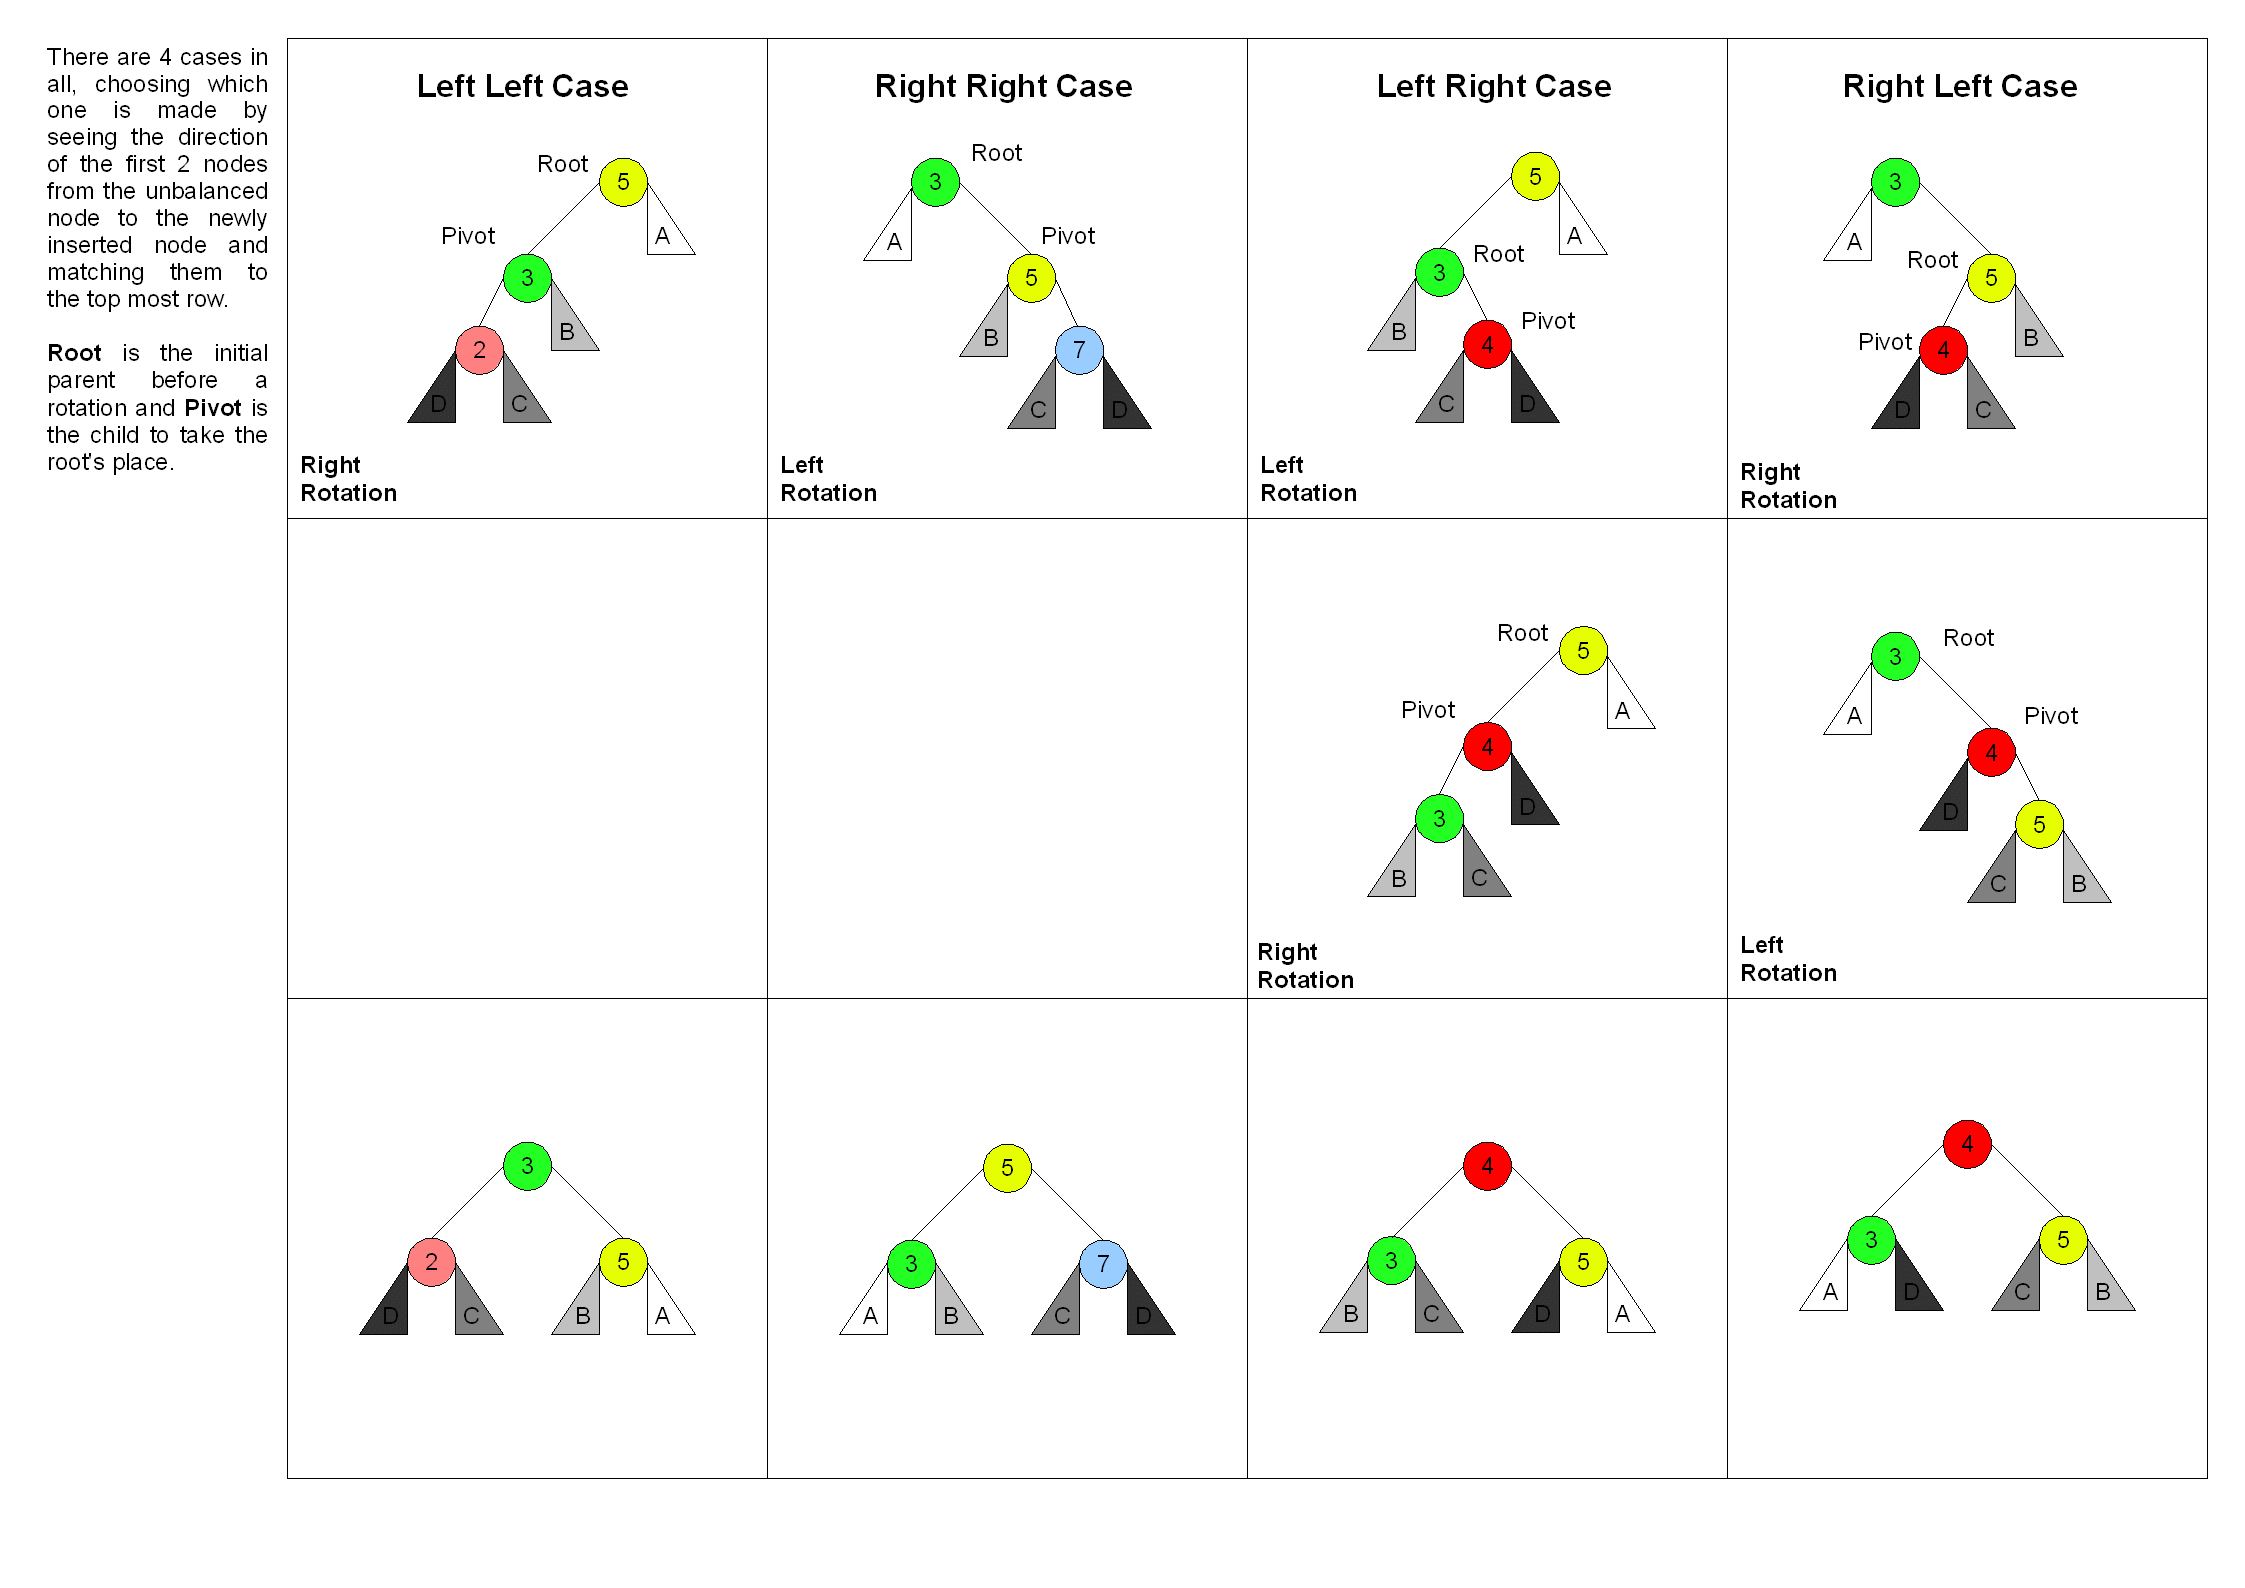
\includegraphics[height=\textheight]{Tree_Rebalancing}
\end{frame}


\subsection{runtime}
\begin{frame}{AVL tree: runtime}
    \begin{itemize}
    \item worst depth of node: $\Theta(\log_2 n + 2) = \Theta(\log n)$
    \item find: $\Theta(\log n)$ 
        \begin{itemize}
            \item worst case: traverse from root to worst depth leaf
        \end{itemize}
    \item insert: $\Theta(\log n)$
        \begin{itemize}
            \item worst case: traverse from root to worst depth leaf \\
                then back up (update balance factors) \\
                then perform constant time rotation
        \end{itemize}
    \item remove: $\Theta(\log n)$
        \begin{itemize}
            \item left as exercise (similar to insert)
        \end{itemize}
    \item print: $\Theta(n)$
        \begin{itemize}
            \item visit each of $n$ nodes
        \end{itemize}
    \end{itemize}
\end{frame}


% R-B trees
\section{red-black trees}

\usetikzlibrary{graphs,graphdrawing}
\usegdlibrary{trees}

\begin{frame}{other types of trees}
    \begin{itemize}
    \item many kinds of \textit{balanced trees}
    \item not all binary trees
    \item different ways of tracking balance factors, etc.
    \item different ways of doing tree rotations or equivalent
    \end{itemize}
\end{frame}

\begin{frame}{red-black trees}
    \begin{itemize}
        \item each node is {\color{red!60!black}\textbf{red}} or \textbf{black}
        \item null leafs considered nodes to aid analysis (still null pointers\ldots)
        \item rules about when nodes can be red/black gaurentee maximum depth
    \end{itemize}
\begin{tikzpicture}
\tikzset{
    >=Latex,
    myt/.style={binary tree layout,level distance=2mm,sibling distance=5mm,nodes={draw,circle,very thick,inner sep=0.25mm,minimum width=1cm,align=center,font=\small,fill=white}},
    R/.style={fill=red!20},
    B/.style={fill=black!90,text=white},
    null/.style={rectangle,draw=none,text=white,label={[font=\small]center:NULL}},
}
\begin{scope}[myt]
\graph {
    [fresh nodes] 13[B] -> {
        8[R] -> {1[B] -> {n[null], 6[R] -> {n[null], n[null]}}, 11[B] -> {n[null], n[null]}},
        17[R] -> {15[B] -> {n[null], n[null]}, 25[B] -> {22[R] -> {n[null], n[null]}, 27[B] -> {n[null], n[null]}}}
    }
};
\end{scope}
\end{tikzpicture}
\end{frame}

\newcommand{\nred}[1]{{\color{red!60!black}\bfseries #1}}

% FIXME: mini version of above figure?
\begin{frame}{red-black tree rules}
    \begin{itemize}
    \item root is \textbf{black}
    \item counting null pointers as nodes, leaves are \textbf{black}
    \item a \nred{red} node's children are \textbf{black}
        \begin{itemize}
            \item $\rightarrow$ a \nred{red} node's parents are \textbf{black}
        \end{itemize}
    \item every simple path from node to leaf under it contains same number of black nodes
            \begin{itemize}
                \item (property holds regardless of whether null pointers are considered nodes)
            \end{itemize}
    \end{itemize}
\end{frame}

% FIXME: why last property limits imbalance

\begin{frame}{worst red-black tree imbalance}
same number of black nodes on paths to leaves \\
    $\rightarrow$ factor of 2 imbalance max \\
\begin{tikzpicture}
\tikzset{
    >=Latex,
    myt/.style={binary tree layout,level distance=2mm,sibling distance=5mm,nodes={draw,circle,very thick,inner sep=0.25mm,minimum width=1cm,align=center,font=\small,fill=white}},
    R/.style={fill=red!20},
    B/.style={fill=black!90,text=white},
    null/.style={rectangle,draw=none,text=white,label={[font=\small]center:NULL}},
}
\begin{scope}[myt]
\graph {
    [fresh nodes] A[B] -> {
        B[B] -> {D[B], E[B]},
        C[R] -> {F[B] -> {H[R] -> {J[B], K[B]}, I[R] -> {L[B], M[B]}}, G[B] -> {N[B], O[B]}}
    }
};
\end{scope}
\end{tikzpicture}
\end{frame}




% FIXME: redraw figures?
\usetikzlibrary{graphs,graphdrawing}
\usegdlibrary{trees}

\begin{frame}<1>[label=rbInsertCases]{red-black insert}
\begin{itemize}
\item default: insert as \nred{red} (no change to black node count), but\ldots
\item \myemph<2>{(1) if new node is root}: color \nblack{black}
\item \myemph<3>{(2) if parent is black}: keep child \nred{red}
\item \myemph<4>{(3) if parent and uncle is \nred{red}}: adjust several colors
\item \myemph<5>{(4) if parent is \nred{red}, uncle is \nblack{black}}, new node is right child
    \begin{itemize}
    \item perform a rotation, then go to case 5
    \end{itemize}
\item \myemph<6>{(5) if parent is \nred{red}, uncle is \nblack{black}}, new node is left child
    \begin{itemize}
    \item perform a rotation
    \end{itemize}
\end{itemize}
\begin{tikzpicture}[overlay, remember picture]
\coordinate (where) at ([yshift=1cm]current page.south);
\tikzset{
    box/.style={draw,very thick,fill=white,at=(where), anchor=south, align=left},
}
\begin{visibleenv}<2>
\node[box] {
    property: ``root is black'' \\
    no children $\rightarrow$ no worries about \# black nodes \\
    on different paths
};
\end{visibleenv}
\begin{visibleenv}<3>
\node[box] {
    property: ``children of \nred{red} node are \nblack{black}'' \\
    no change in \# of \nblack{black} nodes on paths 
};
\end{visibleenv}
\end{tikzpicture}
\end{frame}

\againframe<3>{rbInsertCases}

\againframe<4>{rbInsertCases}

\begin{frame}{case 3: parent, uncle are red}
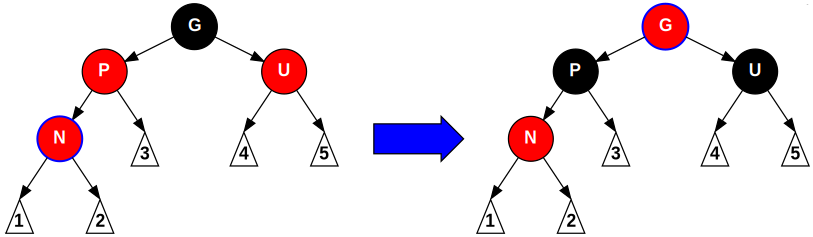
\includegraphics[width=0.9\textwidth]{Red-black_tree_insert_case_3}
\begin{itemize}
\item make grandparent \nred{red}, parent and uncle \nblack{black}
    \begin{itemize}
    \item (property: every path to leaf has same number of black nodes)
    \item just swapped grandparent and parent/uncle in those paths
    \end{itemize}
\item<2-> but\ldots what if grandparent's parent is red?
    \begin{itemize}
    \item (property: children of red node are black)
    \item solution: \myemph<3>{recurse to the grandparent}, as if it was just inserted
    \end{itemize}
\end{itemize}
    \imagecredit{image: Wikipedia/Abloomfi}
\end{frame}

\againframe<5>{rbInsertCases}

\begin{frame}{case 4: parent red, uncle black, right child}
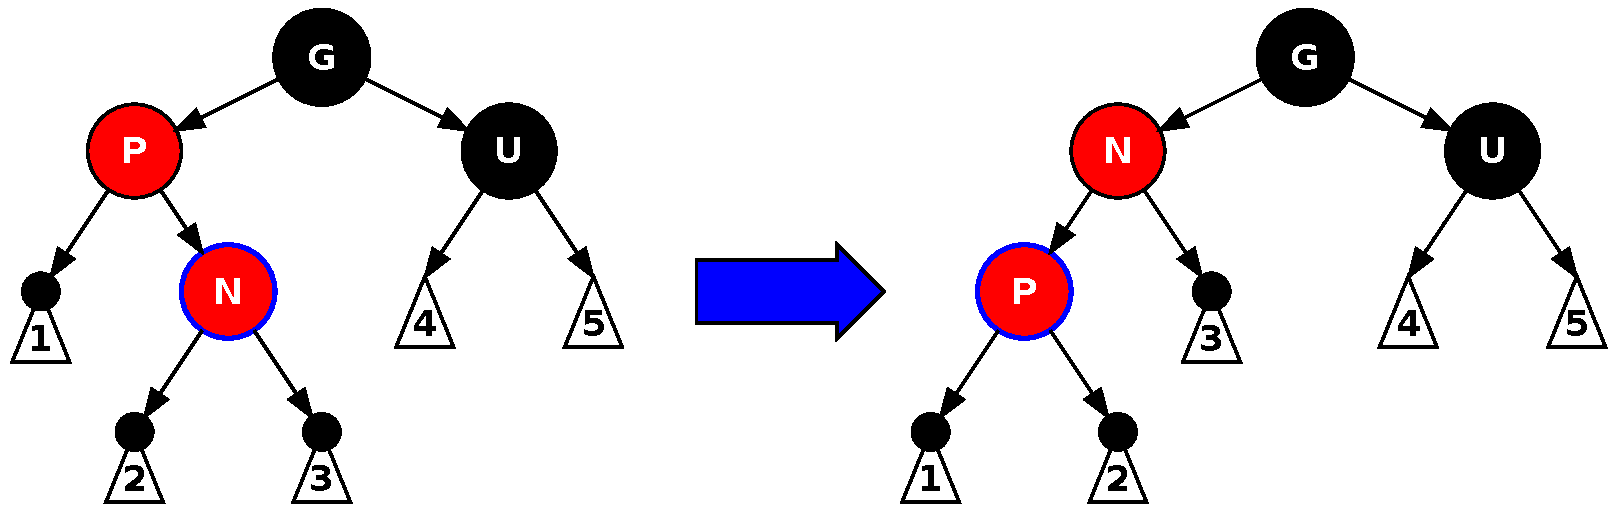
\includegraphics[width=0.9\textwidth]{Red-black_tree_insert_case_4}
\begin{itemize}
\item perform left rotation on parent subtree and new node
\item now case 5 (but new node is $P$, not $N$)
\end{itemize}
    \imagecredit{image: Wikipedia/Abloomfi}
\end{frame}

\againframe<6>{rbInsertCases}

\begin{frame}{case 5: parent red, uncle black, left child}
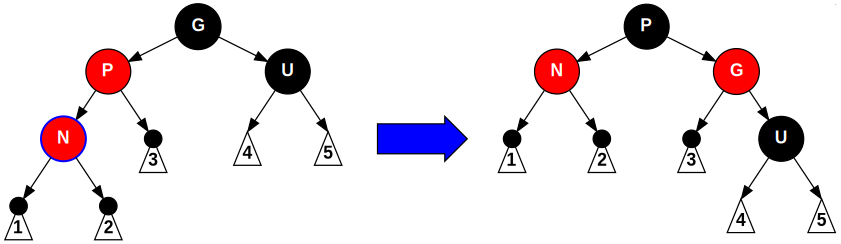
\includegraphics[width=0.9\textwidth]{Red-black_tree_insert_case_5}
\begin{itemize}
\item perform right rotation of grandparent and parent
\item swap colors of parent and grandparent
\item preserves properties:
\begin{itemize}
\item red parent's children are black
\item every path to leaf has same number of black nodes
\end{itemize}
\end{itemize}
    \imagecredit{image: Wikipedia/Abloomfi}
\end{frame}

\begin{frame}{example recursive case}
\begin{tikzpicture}
\tikzset{
    >=Latex,
    myt/.style={binary tree layout,level distance=2mm,sibling distance=25mm,nodes={draw,circle,very thick,inner sep=0.25mm,minimum width=1cm,align=center,font=\small,fill=white}},
    mytB/.style={myt,nodes={draw,circle,very thick,inner sep=0.25mm,minimum width=1cm,align=center,font=\small,fill=white}},
    R/.style={fill=red!20},
    B/.style={fill=black!90,text=white},
    null/.style={rectangle,draw=none,text=white,label={[font=\small]center:NULL}},
    inserted/.style={alt=<1-3>{draw=blue,ultra thick}},
    insertedB/.style={alt=<4-6>{draw=blue,ultra thick}},
    hiParUncle/.style={alt=<2-3>{draw=red,ultra thick,dashed}},
    hiParUncleB/.style={alt=<4-5>{draw=red,ultra thick,dashed}}
}
\begin{visibleenv}<1-4>
\begin{scope}[myt]
\graph {
    [fresh nodes,name=g] 100[B] -> {
        10[R,hiParUncleB] -> { 3[alt=<1-2>{B},alt=<3-4>{R},insertedB] -> {1[alt=<1-2>{R},alt=<3-4>{B},hiParUncle], 5[alt=<1-2>{R},alt=<3-4>{B},hiParUncle] ->[alt=<1>{white}] 8[second,inserted,R,alt=<1>{white}]}, 15[B] },
        200[B,hiParUncleB]
    }
};
\end{scope}
\end{visibleenv}
\begin{visibleenv}<5->
\begin{scope}[myt,sibling distance=15mm]
\graph {
    [fresh nodes,name=gB] 10[B] -> {
        3[R] -> {1[B], 5[B] -> 8[R,second]},
        100[R] -> {15[B], 200[B]}
    }
};
\end{scope}
\end{visibleenv}
\tikzset{
    box/.style={left=2cm of g 100,draw,thick,align=left},
}
\begin{visibleenv}<1>
    \node[box] {initially: \\
        leaves are \nblack{black} \checkmark \\
        \nred{red} node's children are \nblack{black} \checkmark \\
        same number of black nodes \\
        in every path from node to leaves \checkmark 
        };
\end{visibleenv}
\begin{visibleenv}<2>
    \node[box] {insert \textbf{\color{blue!70!black}8} \\
    initially make \nred{red} \\
    \myemph{case 3: parent, uncle are red}};
\end{visibleenv}
\begin{visibleenv}<3>
    \begin{scope}[mytB]
\graph {
    [fresh nodes,name=alt3] 3[B,desired at={([xshift=-6cm]g 3)}] -> { 1[R,hiParUncle], 5[R,hiParUncle] -> 8[R,second,inserted] }
};
    \end{scope}
    \node[above=0cm of alt3 3] {\textit{before:}};
    \draw[Latex-] (alt3 3.north east) -- ++(.5cm,.5cm);
    \node[box] {\myemph{case 3: parent, uncle are red}: \\
    grandparent becomes \nred{red} \\
    parent/uncle \nblack{black}
    };
\end{visibleenv}
\begin{visibleenv}<4>
    \node[box] {case 3 (parent, uncle are red) continued: \\
        recusively examine grandparent \textbf{\color{blue!70!black}3} \\
        \myemph{case 4: parent (of 3) is red} \\
        \hspace{1cm}\myemph{uncle is black, left child}
    };
\end{visibleenv}
\begin{visibleenv}<5>
    \begin{scope}[mytB]
\graph {
    [fresh nodes,name=alt5] 100[B,desired at={([xshift=-8cm,yshift=1cm]gB 10)}] -> {10[R] -> {3[R] -> {"\ldots"[draw=none],"\ldots"[draw=none]}, 15[B]},
        200[B]}
};
    \end{scope}
    \node[draw,thick,align=left,below=1cm of alt5 15] {\myemph{case 4: parent is red} \\
    \hspace{1cm}\myemph{uncle is black, left child}: \\
        perform right rotation \\ of parent + grandparent (of 3) \\
        (and swap parent/grandparent colors)
    };
    \draw[line width=.5mm,-Latex] ([xshift=1cm]alt5 200.east) -- ++(2cm,0cm);
\end{visibleenv}
\end{tikzpicture}
\end{frame}



\begin{frame}{RB-tree: removal}
\begin{itemize}
\item start with normal BST remove of $x$, but\ldots
\item instead find next highest/lowest node $y$
    \begin{itemize}
    \item can choose node \textit{with at most one child} \\
            (``bottom'' of a left or right subtree)
    \end{itemize}
\item swap $x$ and $y$'s value, then replace $y$ with its child
\vspace{.5cm}
\item several cases for color maintainence/rotations
\end{itemize}
\end{frame}

\begin{frame}{RB tree: removal cases}
\begin{itemize}
\item N: node just replaced with child; S: its sibling; P: its parent
\vspace{.5cm}
\item (1): N is new root
\item (2): S is \nred{red}
\item (3): P, S, and S's children are \nblack{black}
\item (4): S and S's children are \nblack{black}
\item (5): S is \nblack{black}, S's left child is \nred{red}, S's right child is \nblack{black}, N is left child of P
\item (6): S is \nblack{black}, S's right child is \nblack{red}, N is left child
\vspace{.5cm}
\item details: see, e.g., Wikipedia article
\end{itemize}
\end{frame}


\begin{frame}{why red-black trees?}
\begin{itemize}
\item a lot more cases\ldots but
\item a lot less rotations
\item \ldots because tree is kept less rigidly balanced
\vspace{.5cm}
\item red-black trees end up being faster in practice
\end{itemize}
\end{frame}


% Splay Trees

% Tree Applications
